% =============================================================
%  PMSM wind generator with finite-set predictive current control and extended Kalman filter:
%  the model mpc_psm of pwr-control/modelization-and-control (foundations_of_power_electronics/mpc_psm)
%  pwr-control documentation - compile with pdflatex (three times) from inside this folder:
%      pdflatex psm_mpc_ekf.tex && pdflatex psm_mpc_ekf.tex && pdflatex psm_mpc_ekf.tex
%  Block diagrams, the state diagram and the torque curve are drawn in this file (TikZ, pgfplots).
%  The numbers of Sections 6.7 and 7 and the two PNG figures come from the companion scripts in py/
%  (python3, numpy, matplotlib; no MATLAB), with the numbers of init_model.m of the model:
%      cd py && python3 design_check_mpc_psm.py ../figures   -> figures/design_check_mpc_psm_output.txt, figures/*.png
%      cd py && python3 ekf_speed_bias.py > ../figures/ekf_speed_bias_output.txt
%  Rev. 01 (November 2026) replaces the whole earlier document of this folder.
% =============================================================
\documentclass[11pt,a4paper]{scrartcl}
% ===================== PACKAGES =====================
\usepackage[british]{babel}
\usepackage[tmargin=1in, bmargin=1in, lmargin=0.75in, rmargin=0.75in]{geometry}
\usepackage[dvipsnames,table]{xcolor}  % prima di tikz, listings, ecc.

\usepackage{tikz}
\usepackage{graphicx}
\usepackage{pgfplots}
\pgfplotsset{width=12cm, compat=1.9}
\usepackage{setspace}
\usepackage{chemmacros}
\usepackage{chemfig}
\usepackage{esint}
\usepackage{tabularray}
\usepackage{makeidx}
\usepackage{epstopdf}
\usepackage{amssymb}
\usepackage{mathrsfs}
\usepackage{bm}
\usepackage{amsmath}
\usepackage{enumitem}
\usepackage[english]{varioref}
\usepackage{lipsum}
\usepackage{fancyhdr}
\usepackage{float}
\usepackage{empheq}
\usepackage[framemethod=tikz]{mdframed}
\numberwithin{equation}{section}
\usepackage{eso-pic}
\usepackage{calc}
\usepackage{nccmath}
\usepackage{caption}
\usepackage{subcaption}
\usepackage{gensymb}
\usepackage{amsfonts, amsthm, epsfig, epstopdf, titling, url, array}
\usepackage{tabularx}
\usepackage{makecell}
\usepackage{booktabs}
\usepackage{array}
\usepackage{siunitx}
\sisetup{input-digits=0123456789\pi}
\usepackage[symbol]{footmisc}
\usepackage{multicol}
\usepackage{boondox-cal}
\usepackage{blindtext}
\usepackage{changepage}
\usepackage{nomencl}
\usepackage{hyperref}
\usepackage{xurl}
\usepackage{ragged2e}
\usepackage[version=4]{mhchem}  % ← conflitto di opzioni
\usepackage{longtable}
\usepackage{chemformula}
\usetikzlibrary{arrows.meta,positioning,calc}

% ===================== SI UNITS =====================
\DeclareSIUnit\atm{atm}
\DeclareSIUnit{\var}{var}
\DeclareSIUnit{\pu}{p.u.}


% ===================== MATH OPERATORS =====================
\DeclareMathOperator{\rank}{rank}
\DeclareMathOperator{\atantwo}{atan2}
\DeclareMathOperator{\spn}{span}

% ===================== COMMANDS =====================
\newcommand{\abs}[1]{\left|#1\right|}
\newcommand{\sign}{\text{sign}}
\newcommand{\centered}[1]{\begin{tabular}{@{}l@{}} #1 \end{tabular}}

% ===================== COLORS =====================
\definecolor{mycolor1}{rgb}{0.97, 0.97, 0.97}
\definecolor{mycolor2}{rgb}{0.97, 0.97, 0.97}
\definecolor{tableShade}{gray}{0.9}

% ===================== THEOREM ENVIRONMENTS =====================
\theoremstyle{it}
\newtheorem{defn}{Definition}[section]
\newtheorem{assumption}{Assumption}[section]
\newtheorem{thm}{Theorem}[section]
\newtheorem{lemma}{Lemma}[section]
\newtheorem{corollary}{Corollary}[section]
\theoremstyle{definition}
\newtheorem{example}{Example}[section]

% ===================== CUSTOM ENVIRONMENTS =====================
\newenvironment{myitemize_1}{
	\begin{itemize}[topsep=0pt]
		\setlength{\topsep}{2pt}
		\setlength{\itemsep}{2pt}
		\setlength{\parskip}{2pt}
		\setlength{\parsep}{2pt}
	}{\end{itemize}}

\newmdenv[
innerlinewidth=0.5pt,
roundcorner=4pt,
backgroundcolor=mycolor2,
linecolor=mycolor1,
innerleftmargin=6pt,
innerrightmargin=6pt,
innertopmargin=6pt,
innerbottommargin=6pt
]{mybox}

% ===================== TABLE COLUMN TYPES =====================
\newcolumntype{Y}{>{\hsize=2\hsize}X}
\newcolumntype{Z}{>{\centering\arraybackslash\hsize=0.857\hsize}X}

% ===================== SECTION DEPTH =====================
\setcounter{secnumdepth}{3}
\setcounter{tocdepth}{3}

% ===================== PAGE STYLE =====================
\setlength{\headheight}{20pt}
\setlength{\headsep}{20pt}

\pagestyle{fancy}
\fancypagestyle{firstpage}{\rhead{}}
\fancyhead[L]{\slshape\nouppercase{\leftmark}}
\chead{}
\rhead{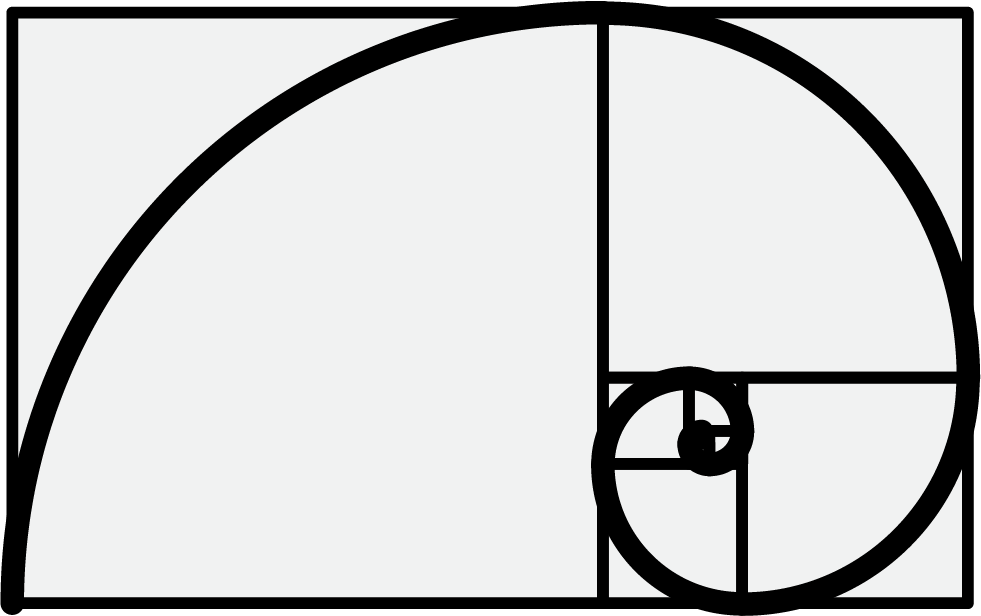
\includegraphics[height=0.75cm]{../../AAA_template_latex_settings/pwr-control_logo_doc.png}}
\lfoot{\href{http://www.pwr-control.com}{pwr-control.com}}
\cfoot{-\ \thepage\ -}
\rfoot{\textit{}}
\renewcommand{\headrulewidth}{0.4pt}
\renewcommand{\footrulewidth}{0.4pt}


\geometry{
	a4paper,
	top    = 2.5cm,
	bottom = 3.0cm,
	left   = 2.5cm,
	right  = 2.5cm
}

\hypersetup{
	colorlinks = true,
	urlcolor   = blue,
	linkcolor  = black,
	citecolor  = black
}

\pagenumbering{gobble}

\usetikzlibrary{shapes.geometric,fit,decorations.pathreplacing}
\pgfplotsset{compat=1.16}

\newcommand{\ped}[1]{_{\mathrm{#1}}}
\newcommand{\code}[1]{\texttt{#1}}
\newcommand{\pun}{\,\mathrm{pu}}
\newcommand{\jj}{\mathrm{j}}
\newcommand{\T}{^{\mathsf{T}}}
\renewcommand{\tabularxcolumn}[1]{>{\raggedright\arraybackslash}p{#1}}
\setlength{\emergencystretch}{3em}
\sisetup{per-mode=symbol,retain-explicit-plus}

% ---------------- document metadata (read by the title page) ----------------
\newcommand{\DocCategory}{Technical Note}
\newcommand{\DocField}{Power Electronics and Control Systems}

\newcommand{\DocTitle}{%
	{\fontsize{20}{24}\selectfont\bfseries PMSM wind generator with predictive\\ current control and extended Kalman filter\par}
	\vspace{14pt}
	{\fontsize{16}{23}\selectfont\bfseries the model \code{mpc\_psm}: two-level inverter, finite-set MPC\\ with delay compensation, sensorless EKF\par}
}

\newcommand{\DocSubtitle}{%
	How the model \code{foundations\_of\_power\_electronics/mpc\_psm} of \code{pwr-control/modelization-and-control} works after the control fixes of November 2026: the machine seen from the bridge, the predictive control and its current loop, the extended Kalman filter and its speed, the torque reference, the parameters and the results of the design check.
}

\newcommand{\DocAuthor}{Davide Bagnara}
\newcommand{\DocRevision}{01}
\newcommand{\DocDate}{November 2026}

\newcommand{\DocAbstract}{%
	The model \code{mpc\_psm} simulates one of the six three-phase systems of a \SI{1.6}{\mega\watt}, \SI{17.8}{rpm}, 104-pole permanent magnet wind generator (about \SI{267}{\kilo\watt} per system) on a two-level inverter with a \SI{230}{\micro\henry} output inductor and a DC link across a \SI{1200}{\volt} lithium-ion battery. A finite-set model predictive control (FCS-MPC) tests the eight states of the bridge every \SI{66.7}{\micro\second} and writes the six gate commands; an extended Kalman filter (EKF) gives the angle and the flux of the rotor without a position sensor, and a double integrator observer on the EKF angle gives the speed. This note describes the model after the control fixes of November 2026: the machine seen from the bridge and its active flux, which makes one inductance ($L_q$ plus the inductor) right for the control; the voltage of the states, the delay compensation and the cost function with its switching term; the current loop seen as a deadbeat loop; the six-state EKF, its state prediction, noise and input timing, and why its speed state is \SI{0.3}{\percent} low with the forward Euler step; the torque reference. A switched simulation of the whole chain checks the design: sensorless angle error \ang{-0.1} (std \ang{0.35}), speed 0.9992, current error \SI{2.8}{\ampere} rms, \SI{2.8}{\kilo\hertz} per device, sensorless from \SI{-25}{\percent} to \SI{+20}{\percent} of the machine inductances. Parameters, files, links to the model and open points close the note.
}

\newcommand{\RevisionHistory}{%
	00 & before Nov.~2026 & The earlier document of this folder: PMSM and induction machine models, EKF, space vector and predictive modulators of an older control (no date; its title was the one of \code{im\_mpc\_ekf}). & \DocAuthor \\
	01 & November 2026 & Complete rewrite on the model \code{mpc\_psm} after the control fixes of November 2026 (modelization-and-control PR \#33); the induction machine part is left out (see \code{im\_mpc\_ekf}); companion scripts of the design check. & \DocAuthor \\
}

\newcommand{\MetaLabelA}{MATLAB model}
\newcommand{\MetaValueAUrl}{https://github.com/pwr-control/modelization-and-control/tree/dev/foundations_of_power_electronics/mpc_psm}
\newcommand{\MetaValueALabel}{modelization-and-control.git (foundations\_of\_power\_electronics/mpc\_psm)}

\newcommand{\MetaLabelB}{Framework}
\newcommand{\MetaValueB}{MATLAB/Simulink, Simscape, GNU Octave, Python}

\begin{document}

% =============================================================
%  pwr-control LaTeX template - FRONTESPIZIO
%
%  Da richiamare come prima istruzione dopo \begin{document}:
%      % =============================================================
%  pwr-control LaTeX template - FRONTESPIZIO
%
%  Da richiamare come prima istruzione dopo \begin{document}:
%      % =============================================================
%  pwr-control LaTeX template - FRONTESPIZIO
%
%  Da richiamare come prima istruzione dopo \begin{document}:
%      \input{../../AAA_template_latex_settings/titlepage}
%
%  Il documento deve definire prima di \begin{document}:
%      \DocCategory   categoria del documento
%      \DocField      area tecnica
%      \DocTitle      titolo (una o due righe)
%      \DocSubtitle   sottotitolo
%      \DocAuthor     autore/i, separati da virgola
%      \DocRevision   numero di revisione corrente (es. 00)
%      \DocDate       data della revisione corrente
%      \DocAbstract   abstract
%      \RevisionHistory  righe della tabella di revisione, nel formato
%                        Rev. & Date & Description & Authors \\
%      \MetaLabelA \MetaValueAUrl \MetaValueALabel
%      \MetaLabelB \MetaValueB
% =============================================================

\providecommand{\DocCategory}{Technical Research Report}
\providecommand{\DocField}{Power Electronics and Control Systems}
\providecommand{\DocSubtitle}{}
\providecommand{\DocRevision}{00}
\providecommand{\DocAbstract}{}
\providecommand{\RevisionHistory}{%
	\DocRevision & \DocDate & First issue. & \DocAuthor \\
}

\titlepage

% ---- Intestazione centrata ----
\begin{center}
	{\Large\scshape \DocCategory}\\[8pt]
	{\large\scshape \DocField}
\end{center}

\vspace{30pt plus 4pt minus 14pt}
\noindent\rule{\linewidth}{0.8pt}

% ---- Titolo ----
\begin{center}
	\DocTitle
\end{center}

\vspace{4pt}
\noindent\rule{\linewidth}{2.2pt}

% ---- Sottotitolo ----
\begin{center}
	\begin{onehalfspace}
		{\large\itshape \DocSubtitle}
	\end{onehalfspace}
\end{center}

% ---- Authors / Revision / Date ----
\vspace{30pt plus 4pt minus 14pt}

\noindent
\begin{minipage}[t]{0.46\linewidth}
	\raggedright
	\textbf{Authors:}\\[2pt]
	\DocAuthor
\end{minipage}%
\hfill
\begin{minipage}[t]{0.22\linewidth}
	\centering
	\textbf{Revision:}\\[2pt]
	\DocRevision
\end{minipage}%
\hfill
\begin{minipage}[t]{0.30\linewidth}
	\raggedleft
	\textbf{Date:}\\[2pt]
	\DocDate
\end{minipage}

\vspace{10pt}
\noindent\rule{\linewidth}{0.8pt}

% ---- Abstract ----
\vspace{24pt plus 4pt minus 12pt}

\begin{center}
	\begin{minipage}{0.88\linewidth}
		\footnotesize
		\begin{onehalfspace}
			\textbf{Abstract:} \DocAbstract
		\end{onehalfspace}
	\end{minipage}
\end{center}

\vfill

% ---- Revision history ----
\begin{center}
	\begin{minipage}{0.96\linewidth}
		\centering
		{\footnotesize\scshape Revision history}\\[6pt]
		{\footnotesize
			\begin{tabular}{@{}cl>{\raggedright\arraybackslash}p{0.36\linewidth}>{\raggedright\arraybackslash}p{0.28\linewidth}@{}}
				\toprule
				\textbf{Rev.} & \textbf{Date} & \textbf{Description} & \textbf{Authors} \\
				\midrule
				\RevisionHistory
				\bottomrule
			\end{tabular}}
	\end{minipage}
\end{center}

\vspace{18pt plus 4pt minus 10pt}

% ---- Metadati in fondo ----
\noindent
\begin{tabular}{@{} r @{\quad} l @{}}
	\textsc{\MetaLabelA:} & {\href{\MetaValueAUrl}{\MetaValueALabel}} \\[3pt]
	\textsc{\MetaLabelB:} & {\MetaValueB}       \\[3pt]
\end{tabular}

% =============================================================
%  Fine frontespizio
% =============================================================
\newpage
\pagenumbering{arabic}
\setcounter{page}{1}

%
%  Il documento deve definire prima di \begin{document}:
%      \DocCategory   categoria del documento
%      \DocField      area tecnica
%      \DocTitle      titolo (una o due righe)
%      \DocSubtitle   sottotitolo
%      \DocAuthor     autore/i, separati da virgola
%      \DocRevision   numero di revisione corrente (es. 00)
%      \DocDate       data della revisione corrente
%      \DocAbstract   abstract
%      \RevisionHistory  righe della tabella di revisione, nel formato
%                        Rev. & Date & Description & Authors \\
%      \MetaLabelA \MetaValueAUrl \MetaValueALabel
%      \MetaLabelB \MetaValueB
% =============================================================

\providecommand{\DocCategory}{Technical Research Report}
\providecommand{\DocField}{Power Electronics and Control Systems}
\providecommand{\DocSubtitle}{}
\providecommand{\DocRevision}{00}
\providecommand{\DocAbstract}{}
\providecommand{\RevisionHistory}{%
	\DocRevision & \DocDate & First issue. & \DocAuthor \\
}

\titlepage

% ---- Intestazione centrata ----
\begin{center}
	{\Large\scshape \DocCategory}\\[8pt]
	{\large\scshape \DocField}
\end{center}

\vspace{30pt plus 4pt minus 14pt}
\noindent\rule{\linewidth}{0.8pt}

% ---- Titolo ----
\begin{center}
	\DocTitle
\end{center}

\vspace{4pt}
\noindent\rule{\linewidth}{2.2pt}

% ---- Sottotitolo ----
\begin{center}
	\begin{onehalfspace}
		{\large\itshape \DocSubtitle}
	\end{onehalfspace}
\end{center}

% ---- Authors / Revision / Date ----
\vspace{30pt plus 4pt minus 14pt}

\noindent
\begin{minipage}[t]{0.46\linewidth}
	\raggedright
	\textbf{Authors:}\\[2pt]
	\DocAuthor
\end{minipage}%
\hfill
\begin{minipage}[t]{0.22\linewidth}
	\centering
	\textbf{Revision:}\\[2pt]
	\DocRevision
\end{minipage}%
\hfill
\begin{minipage}[t]{0.30\linewidth}
	\raggedleft
	\textbf{Date:}\\[2pt]
	\DocDate
\end{minipage}

\vspace{10pt}
\noindent\rule{\linewidth}{0.8pt}

% ---- Abstract ----
\vspace{24pt plus 4pt minus 12pt}

\begin{center}
	\begin{minipage}{0.88\linewidth}
		\footnotesize
		\begin{onehalfspace}
			\textbf{Abstract:} \DocAbstract
		\end{onehalfspace}
	\end{minipage}
\end{center}

\vfill

% ---- Revision history ----
\begin{center}
	\begin{minipage}{0.96\linewidth}
		\centering
		{\footnotesize\scshape Revision history}\\[6pt]
		{\footnotesize
			\begin{tabular}{@{}cl>{\raggedright\arraybackslash}p{0.36\linewidth}>{\raggedright\arraybackslash}p{0.28\linewidth}@{}}
				\toprule
				\textbf{Rev.} & \textbf{Date} & \textbf{Description} & \textbf{Authors} \\
				\midrule
				\RevisionHistory
				\bottomrule
			\end{tabular}}
	\end{minipage}
\end{center}

\vspace{18pt plus 4pt minus 10pt}

% ---- Metadati in fondo ----
\noindent
\begin{tabular}{@{} r @{\quad} l @{}}
	\textsc{\MetaLabelA:} & {\href{\MetaValueAUrl}{\MetaValueALabel}} \\[3pt]
	\textsc{\MetaLabelB:} & {\MetaValueB}       \\[3pt]
\end{tabular}

% =============================================================
%  Fine frontespizio
% =============================================================
\newpage
\pagenumbering{arabic}
\setcounter{page}{1}

%
%  Il documento deve definire prima di \begin{document}:
%      \DocCategory   categoria del documento
%      \DocField      area tecnica
%      \DocTitle      titolo (una o due righe)
%      \DocSubtitle   sottotitolo
%      \DocAuthor     autore/i, separati da virgola
%      \DocRevision   numero di revisione corrente (es. 00)
%      \DocDate       data della revisione corrente
%      \DocAbstract   abstract
%      \RevisionHistory  righe della tabella di revisione, nel formato
%                        Rev. & Date & Description & Authors \\
%      \MetaLabelA \MetaValueAUrl \MetaValueALabel
%      \MetaLabelB \MetaValueB
% =============================================================

\providecommand{\DocCategory}{Technical Research Report}
\providecommand{\DocField}{Power Electronics and Control Systems}
\providecommand{\DocSubtitle}{}
\providecommand{\DocRevision}{00}
\providecommand{\DocAbstract}{}
\providecommand{\RevisionHistory}{%
	\DocRevision & \DocDate & First issue. & \DocAuthor \\
}

\titlepage

% ---- Intestazione centrata ----
\begin{center}
	{\Large\scshape \DocCategory}\\[8pt]
	{\large\scshape \DocField}
\end{center}

\vspace{30pt plus 4pt minus 14pt}
\noindent\rule{\linewidth}{0.8pt}

% ---- Titolo ----
\begin{center}
	\DocTitle
\end{center}

\vspace{4pt}
\noindent\rule{\linewidth}{2.2pt}

% ---- Sottotitolo ----
\begin{center}
	\begin{onehalfspace}
		{\large\itshape \DocSubtitle}
	\end{onehalfspace}
\end{center}

% ---- Authors / Revision / Date ----
\vspace{30pt plus 4pt minus 14pt}

\noindent
\begin{minipage}[t]{0.46\linewidth}
	\raggedright
	\textbf{Authors:}\\[2pt]
	\DocAuthor
\end{minipage}%
\hfill
\begin{minipage}[t]{0.22\linewidth}
	\centering
	\textbf{Revision:}\\[2pt]
	\DocRevision
\end{minipage}%
\hfill
\begin{minipage}[t]{0.30\linewidth}
	\raggedleft
	\textbf{Date:}\\[2pt]
	\DocDate
\end{minipage}

\vspace{10pt}
\noindent\rule{\linewidth}{0.8pt}

% ---- Abstract ----
\vspace{24pt plus 4pt minus 12pt}

\begin{center}
	\begin{minipage}{0.88\linewidth}
		\footnotesize
		\begin{onehalfspace}
			\textbf{Abstract:} \DocAbstract
		\end{onehalfspace}
	\end{minipage}
\end{center}

\vfill

% ---- Revision history ----
\begin{center}
	\begin{minipage}{0.96\linewidth}
		\centering
		{\footnotesize\scshape Revision history}\\[6pt]
		{\footnotesize
			\begin{tabular}{@{}cl>{\raggedright\arraybackslash}p{0.36\linewidth}>{\raggedright\arraybackslash}p{0.28\linewidth}@{}}
				\toprule
				\textbf{Rev.} & \textbf{Date} & \textbf{Description} & \textbf{Authors} \\
				\midrule
				\RevisionHistory
				\bottomrule
			\end{tabular}}
	\end{minipage}
\end{center}

\vspace{18pt plus 4pt minus 10pt}

% ---- Metadati in fondo ----
\noindent
\begin{tabular}{@{} r @{\quad} l @{}}
	\textsc{\MetaLabelA:} & {\href{\MetaValueAUrl}{\MetaValueALabel}} \\[3pt]
	\textsc{\MetaLabelB:} & {\MetaValueB}       \\[3pt]
\end{tabular}

% =============================================================
%  Fine frontespizio
% =============================================================
\newpage
\pagenumbering{arabic}
\setcounter{page}{1}


\tableofcontents
\listoffigures
\listoftables
\newpage

\begin{onehalfspace}

% =============================================================
\section*{Nomenclature}
\addcontentsline{toc}{section}{Nomenclature}
\label{sec:nomenclature}

\begingroup
\rowcolors{2}{tableShade}{white}
\begin{longtable}{@{} l p{0.76\linewidth} @{}}
	\toprule
	\textbf{Symbol} & \textbf{Meaning} \\
	\midrule
	\endfirsthead
	\toprule
	\textbf{Symbol} & \textbf{Meaning} \\
	\midrule
	\endhead
	\bottomrule
	\endfoot
	\bottomrule
	\endlastfoot
	PMSM & permanent magnet synchronous machine \\
	FCS-MPC & finite-set model predictive control: at every step it tests the states of the bridge and applies the best one \\
	EKF & extended Kalman filter \\
	DIO & double integrator observer: angle and speed from an angle signal \\
	pu & per unit of the machine (one system): voltages in $u\ped{bez}$, currents in $i\ped{bez}$, time in $1/\omega\ped{bez}$ \\
	$u\ped{bez}$, $i\ped{bez}$ & base voltage (peak phase voltage at rated speed, $\psi\ped{m}\,\omega\ped{bez}$) and base current (peak rated phase current) of one system \\
	$\omega\ped{bez}$, $\tau\ped{bez}$ & electrical base pulsation (rated speed) and base torque of one system \\
	$L\ped{bez}$, $X\ped{bez}$ & base inductance and impedance, $X\ped{bez} = u\ped{bez}/i\ped{bez} = \omega\ped{bez}L\ped{bez}$ \\
	$u\ped{dc,nom}$ & \SI{1070}{\volt}, base of the measured DC voltage $v\ped{dc}$ (data set \code{inv690V\_250kW}) \\
	$k_u$ & $u\ped{dc,nom}/u\ped{bez} = 2.925$, from pu of $u\ped{dc,nom}$ to pu of $u\ped{bez}$ (\code{u\_scale}) \\
	$\alpha\beta$, $dq$ & stationary frame (amplitude-invariant Clarke transformation) and rotor frame ($d$ on the magnet axis) \\
	$\underline{x}$ & space vector $x_\alpha + \jj x_\beta$; $\jj\underline{x}$ is $\underline{x}$ turned by \ang{90} \\
	$\underline{u}$, $\underline{i}$, $\underline{e}$ & voltage of the bridge, current, back-EMF \\
	$\psi\ped{m}$, $\underline{\psi}$ & magnet flux; flux of the control model (the active flux, Section~\ref{sec:activeflux}) \\
	$\theta$, $\omega$ & electrical angle and electrical speed (pu of $\omega\ped{bez}$) of the rotor \\
	$L_d$, $L_q$, $R_s$ & inductances and resistance of the machine (one system) \\
	$L\ped{Fi}$, $R\ped{LFi}$ & output inductor of the inverter and its resistance \\
	$L$, $R$ & inductance and resistance of the control model: $L = L_q + L\ped{Fi}$, $R = R_s + R\ped{LFi}$ (\code{L\_norm}, \code{R\_norm}) \\
	$t\ped{s}$, $k$ & control step (\SI{66.7}{\micro\second}) and its index; $t_k$ is the time of step $k$ \\
	$h$ & control step in per-unit time, $h = t\ped{s}\,\omega\ped{bez} = 0.00646$ (\code{ts\_pu}) \\
	$\hat\gamma$ & coefficient of the prediction, $h/L = 0.00644$ (variable \code{g} of the code) \\
	$g$ & gain of the current loop: true current change over predicted current change for the same voltage \\
	$s = (s_a, s_b, s_c)$ & state of the bridge: $s_x = 1$ when the upper switch of leg $x$ is on, 0 when the lower one is on \\
	$J$, $N\ped{sw}$ & cost of a state; number of legs that change state \\
	$k\ped{i}$, $k\ped{sw}$ & weights of the current error and of $N\ped{sw}$ (\code{k\_kalman}, \code{k\_sw}) \\
	$\bm{x}$, $\bm{y}$ & state $[i_\alpha\; i_\beta\; \psi_\alpha\; \psi_\beta\; \omega\; \tau\ped{L}]\T$ and output $[i_\alpha\; i_\beta]\T$ of the EKF \\
	$A_1 \ldots A_6$, $B$, $C$ & coefficient matrices of the Jacobian, input matrix and output matrix of the EKF model \\
	$F\ped{pred}$, $F\ped{cov}$ & transition matrix of the state prediction and of the covariance prediction \\
	$P$, $K$ & covariance of the state error and Kalman gain (the block calls the gain \code{L(k)}) \\
	$Q\ped{K}$, $R\ped{K}$ & process and measurement noise covariances (\code{Qkalman}, \code{Rkalman}) \\
	$q\ped{ekf}$, $r\ped{ekf}$, $j\ped{m}$ & noise weights and inertia of the EKF model (\code{q\_ekf}, \code{r\_ekf}, \code{jm\_ekf}) \\
	$k_\theta$, $k_\omega$ & gains of the double integrator observer \\
	$T$ & electromagnetic torque (pu of $\tau\ped{bez}$) \\
\end{longtable}
\endgroup
\addtocounter{table}{-1}

% =============================================================
\section{Introduction}
\label{sec:intro}

The model \code{mpc\_psm} \cite{mc_repo} belongs to the folder \code{foundations\_of\_power\_electronics} of \code{pwr-control/modelization-and-control}. It simulates one of the six three-phase systems of a permanent magnet wind generator (data set WindGen: \SI{1.6}{\mega\watt}, \SI{17.8}{rpm}, 104 poles, about \SI{267}{\kilo\watt} per system) with its two-level inverter, its DC link and a lithium-ion battery (Figure~\ref{fig:overview}). The shaft turns at a fixed speed and the torque reference follows the torque curve of the turbine. The control runs every \SI{66.7}{\micro\second} (\SI{15}{\kilo\hertz}) in the per unit of the machine and has no modulator: a finite-set model predictive control (FCS-MPC) \cite{kouro2009,rodriguez2012} tests the eight states of the bridge and writes the six gate commands. The angle and the flux of the rotor come from an extended Kalman filter (EKF) on the measured currents, without a position sensor; the speed comes from a double integrator observer (DIO) on the EKF angle.

This note describes the model as it is in the branch \code{dev} after the control fixes of November 2026 (pull request \#33 of modelization-and-control). It replaces the earlier document of this folder, which described an older version of the control and mixed the PMSM with the induction machine; the induction machine is in the document \code{repos\_doc/im\_mpc\_ekf} and in the note \code{research/power\_electronics/im\_foc\_ekf\_sensorless} of this repository. The sibling model \code{mpc\_ttype\_psm} (same machine, three-level T-type bridge) is described in \code{research/power\_electronics/fcs\_mpc\_ttype\_psm} \cite{ttype_note}.

\begin{table}[H]
	\centering
	\footnotesize
	\caption{Where to find the model.}
	\label{tab:links}
	\rowcolors{2}{tableShade}{white}
	\begin{tabularx}{\textwidth}{@{} l X @{}}
		\toprule
		\textbf{What} & \textbf{Link} \\
		\midrule
		model folder (branch \code{dev}) & \url{https://github.com/pwr-control/modelization-and-control/tree/dev/foundations_of_power_electronics/mpc_psm} \\
		README of the model & \url{https://github.com/pwr-control/modelization-and-control/blob/dev/foundations_of_power_electronics/mpc_psm/README.md} \\
		init (live script) & \code{init\_model.m} in the model folder: run it from that folder (Section~\ref{sec:files}) \\
		model & \code{mpc\_psm.slx}; the predictive control is \code{inner\_ctrl/mp control/mpc\_pu\_d} (MATLAB Function \code{mpc}), the EKF is \code{EKF\_bemf\_observer/extended\_kalman\_observer} \\
		library & \url{https://github.com/pwr-control/library} (blocks of the power stage and of the battery) \\
		\bottomrule
	\end{tabularx}
\end{table}

Section~\ref{sec:model} describes the model and the timing of one control step, Section~\ref{sec:machine} the machine seen from the bridge in per unit, Section~\ref{sec:mpc} the predictive control, Section~\ref{sec:reference} the torque and current reference, Section~\ref{sec:ekf} the EKF and the speed, Section~\ref{sec:check} the design check, Section~\ref{sec:history} what changed in November 2026, Section~\ref{sec:params} the parameters, Section~\ref{sec:files} the files and how to run the model, Section~\ref{sec:open} the open points. Appendix~\ref{app:mpc} lists the function \code{mpc} of the model.

\begin{figure}[H]
	\centering
	\resizebox{\textwidth}{!}{%
	\begin{tikzpicture}[font=\scriptsize, >=Latex,
		pw/.style={draw, thick, rounded corners=2pt, fill=blue!8, minimum width=2.3cm, minimum height=1.0cm, align=center},
		ct/.style={draw, thick, rounded corners=2pt, fill=orange!15, minimum width=2.5cm, minimum height=1.0cm, align=center},
		lab/.style={font=\scriptsize, inner sep=1.5pt, fill=white, align=center}]
		% power stage
		\node[pw] (bat) at (0,0) {Li-ion battery\\\SI{1249}{\volt} open circuit};
		\node[pw] (dc) at (3,0) {DC link\\$2\times\SI{14.4}{\milli\farad}$};
		\node[pw] (br) at (6,0) {two-level bridge\\ideal switches};
		\node[pw] (lf) at (10,0) {inductor\\\SI{230}{\micro\henry}};
		\node[pw] (pm) at (13,0) {PMSM\\one of six systems};
		\node[pw] (sh) at (16,0) {shaft\\fixed speed};
		\draw[very thick] (bat) -- (dc); \draw[very thick] (dc) -- (br); \draw[very thick] (br) -- (lf);
		\draw[very thick] (lf) -- (pm); \draw[very thick, double] (pm) -- (sh);
		% control
		\node[ct] (tc) at (0,-2.6) {torque curve\\\SI{1}{\hertz} speed filter};
		\node[ct] (cr) at (3,-2.6) {current reference\\$i_d^* = 0$, $i_q^*$ at $\theta\ped{c}$};
		\node[ct] (mpc) at (6,-2.6) {FCS-MPC \code{mpc}\\8 states, \SI{15}{\kilo\hertz}};
		\node[ct] (acq) at (10,-2.6) {acquisition\\one step late};
		\node[ct] (ekf) at (10,-4.6) {EKF\\6 states};
		\node[ct] (dio) at (13,-4.6) {DIO\\angle $\rightarrow$ speed};
		\node[ct] (sw) at (3,-4.6) {encoder--sensorless\\switch};
		% signals
		\draw[->] (lf.south) -- node[lab]{$i_{uvw}$, $v\ped{dc}$} (acq.north);
		\draw[->] (acq.west) -- node[lab, above=1pt]{$\underline{i}$, $v\ped{dc}$} (mpc.east);
		\draw[->] (acq.south) -- node[lab]{$\underline{i}(t_{k-1})$} (ekf.north);
		\draw[->] (mpc.north) -- node[lab]{6 gates} (br.south);
		\draw[->] (tc.east) -- node[lab, above=1pt]{$i_q^*$} (cr.west);
		\draw[->] (cr.east) -- node[lab, above=1pt]{$\underline{i}^*$} (mpc.west);
		\draw[->] (mpc.south) |- node[lab, pos=0.7]{$\underline{u}_{k-2}$ (Unit Delay)} (ekf.west);
		\draw[->] (ekf.north west) -- node[lab, sloped, above=1pt]{$\hat{\underline{\psi}}$, $\hat\omega$} (mpc.south east);
		\draw[->] (ekf.east) -- node[lab, above=1pt]{$\hat\theta$} (dio.west);
		\draw[->] (dio.south) -- ++(0,-0.7) -| node[lab, pos=0.25]{$\hat\theta$, $\hat\omega$ (sensorless)} (sw.south);
		\draw[->] (sw.north) -- node[lab]{$\theta\ped{c}$} (cr.south);
		\draw[->] (sw.west) -| node[lab, pos=0.75]{$\omega\ped{c}$} (tc.south);
		\draw[<-] ([xshift=-7mm]sw.south) -- ++(0,-0.7) node[below, font=\scriptsize]{encoder (DIO)};
	\end{tikzpicture}}
	\caption{The model \code{mpc\_psm}: power stage (top) and control (bottom). The control runs every $t\ped{s} = \SI{66.7}{\micro\second}$ in pu of the machine; $\underline{u}_{k-2}$ is the voltage of the vector applied two steps before.}
	\label{fig:overview}
\end{figure}

% =============================================================
\section{The model}
\label{sec:model}

\subsection{Power stage}

Table~\ref{tab:power} lists the blocks of the power stage. The bridge is the library block \code{Three-Phase Bridge (ideal)} \cite{library_repo} with its built-in DC capacitor and AC inductors switched off: the model has its own DC link and output inductor. The gate generator \code{dead\_time\_generator\_cmos\_simulink} filters the six gates with the time constant $t\ped{c}$ and puts the dead time between the two switches of a leg: the switch that turns on waits until an RC copy (time constant $\sqrt2\cdot\SI{3}{\micro\second}$) of the other gate is below \SI{7.5}{\volt}, so the bridge sees $\ln 2\cdot\sqrt2\cdot\SI{3}{\micro\second} = \SI{2.94}{\micro\second}$. The solver is \code{ode23tb}; its maximum step and the step of the Simscape local solver are $t\ped{c} = \SI{0.333}{\micro\second}$, with 5 nonlinear iterations, and the simulation starts from the steady state, so the DC link starts at the battery voltage.

\begin{table}[H]
	\centering
	\footnotesize
	\caption{Power stage of \code{mpc\_psm.slx} (one system of the generator).}
	\label{tab:power}
	\rowcolors{2}{tableShade}{white}
	\begin{tabularx}{\textwidth}{@{} >{\raggedright\arraybackslash}p{4.6cm} X @{}}
		\toprule
		\textbf{Block} & \textbf{What it is, data} \\
		\midrule
		\code{battery/lithium\_ion\_battery} & library lithium-ion battery across the whole DC link: 332 cells, \SI{1200}{\volt} nominal, \SI{250}{\kilo\watt}, \SI{1249}{\volt} open circuit at state of charge 0.85; $R_0 = \SI{72}{\milli\ohm}$, $R_1 = \SI{72}{\milli\ohm}$, $C_1 = \SI{10}{\milli\farad}$ (legacy changes: $R_0$, $R_1$ halved, $C_1/50$) \\
		\code{inv\_psm\_mod1/dclink} & \code{dclink\_with\_center\_tap}: $2\times\SI{14.4}{\milli\farad}$ in series, \SI{107}{\kilo\ohm} across each capacitor; gives $v\ped{dc}$ in pu of $u\ped{dc,nom} = \SI{1070}{\volt}$ \\
		\code{inv\_psm\_mod1/inverter} & \code{Three-Phase Bridge (ideal)}: six ideal switches with antiparallel diodes, $R\ped{on} = \SI{1}{\milli\ohm}$, gate threshold \SI{2.5}{\volt}, gate order a+, a$-$, b+, b$-$, c+, c$-$; built-in passives off; the gate generator gives \SI{2.94}{\micro\second} of dead time; the \code{timer} (\SI{15}{\kilo\hertz}, single update) triggers the control \\
		\code{inv\_psm\_mod1/}\newline\code{inverter\_output\_filter} & three-phase inductor, $L\ped{Fi} = \SI{230}{\micro\henry}$, $R\ped{LFi} = \SI{1.8}{\milli\ohm}$ \\
		\code{psm} & library \code{permanent\_magnet\_synchronous\_machine}, one system: $R_s = \SI{30.1}{\milli\ohm}$, $L_d = \SI{6.24}{\milli\henry}$, $L_q = \SI{7.56}{\milli\henry}$, $\psi\ped{m} = \SI{3.774}{\volt\second}$, 104 poles \\
		\code{fixed\_speed\_setting} & ideal speed source: step to \SI{17.8}{rpm} at \SI{25}{\milli\second} through a \SI{0.1}{\second} lag (energy production, default) \\
		\code{motor\_load\_setting} & inertia and load torque, for the speed-control variant (not the default) \\
		\bottomrule
	\end{tabularx}
\end{table}

\subsection{Control chain}
\label{sec:chain}

The control is in the subsystem \code{inv\_psm\_mod1/inverter\_control}; it is triggered every $t\ped{s}$ by the timer and works in pu of the machine of one system:
\begin{enumerate}[nosep]
	\item \textbf{Acquisition.} Phase currents and DC voltage are quantized ($2^{-11}\pun$) and delayed by one step (Unit Delay); encoder angle and speed are quantized (12 bit) and delayed by one step.
	\item \textbf{Torque reference} (\code{torque\_reference}): the speed of the control through a \SI{1}{\hertz} low-pass filter, the torque curve of the turbine, $-1/\tau\ped{bez}$: the $q$ current reference, with $i_d^* = 0$ (Section~\ref{sec:reference}). Variant: speed PI (\code{use\_speed\_control}).
	\item \textbf{Current reference} (\code{current\_reference\_generator}): $i_q^*$ turned to $\alpha\beta$ with the control angle $\theta\ped{c}$.
	\item \textbf{Predictive control} (\code{inner\_ctrl/mp control/mpc\_pu\_d}, MATLAB Function \code{mpc}, Section~\ref{sec:mpc}): chooses one of the eight states, writes the six gates and gives the observers the voltage of the vector applied before.
	\item \textbf{Observers} (\code{bemf\_observer1}): the EKF (default, Section~\ref{sec:ekf}) or one of two back-EMF observers (Simulink, C-Caller); the predictive control always takes flux and speed from the EKF block, whose speed output comes from the DIO on the EKF angle.
	\item \textbf{Encoder--sensorless switch}: angle and speed for the torque curve and the current reference, from the encoder (through a DIO) or from the EKF block (\code{use\_psm\_encoder} = 0, sensorless, by default; the encoder is used while the speed is zero).
	\item \textbf{Timing}: the local clock \code{global timing/time\_inv1} has the gain 1.001 (open point~\ref{op:clock}); its alignment loop \code{phase\_compensation\_1} has zero gains.
\end{enumerate}

\subsection{Timing of one control step}
\label{sec:timing}

Figure~\ref{fig:timing} shows what happens at step $k$. The current and the DC voltage sampled at $t_{k-1}$ are used at step $k$. The vector $\underline{u}_k$ chosen at step $k$ acts over $[t_k, t_{k+1})$, so it decides the current at $t_{k+1}$, while $\underline{u}_{k-1}$ is still acting when $\underline{u}_k$ is chosen: the control first computes the current of now with $\underline{u}_{k-1}$ (delay compensation, Section~\ref{sec:prediction}). The current measured at step $k$ was made by $\underline{u}_{k-2}$, which is the voltage the EKF needs with that current (Section~\ref{sec:ekftiming}). The outputs of the EKF are read from its state memory: at step $k$ they are the estimate of $t_{k-2}$.

\begin{figure}[H]
	\centering
	\begin{tikzpicture}[x=2.8cm, y=1cm, >=Stealth, font=\small]
		\draw[->] (-0.25,0) -- (4.4,0) node[right]{$t$};
		\foreach \x/\l in {0/t_{k-2},1/t_{k-1},2/t_k,3/t_{k+1},4/t_{k+2}} {\draw (\x,0.08) -- (\x,-0.08) node[below]{$\l$};}
		\fill[blue!12] (0,0.25) rectangle (1,0.75); \node at (0.5,0.5) {$\underline{u}_{k-2}$};
		\fill[blue!12] (1,0.25) rectangle (2,0.75); \node at (1.5,0.5) {$\underline{u}_{k-1}$};
		\fill[orange!30] (2,0.25) rectangle (3,0.75); \node at (2.5,0.5) {$\underline{u}_{k}$};
		\draw[white, line width=1pt] (1,0.25) -- (1,0.75) (2,0.25) -- (2,0.75);
		\draw[->, thick] (1,1.15) -- (1,0.8);
		\node[above, align=center] at (1,1.15) {sample $\underline{i}$, $v\ped{dc}$};
		\node[draw, rounded corners, align=left, fill=white, font=\footnotesize] (stepk) at (2.9,2.55) {step $k$: \textbf{1.} read the EKF outputs (estimate of $t_{k-2}$);\\ \textbf{2.} $\hat{\underline{i}}(t_k)$ from $\underline{i}(t_{k-1})$ and $\underline{u}_{k-1}$; \textbf{3.} choose $\underline{u}_k$ for $\underline{i}(t_{k+1})$;\\ \textbf{4.} EKF step with $\underline{i}(t_{k-1})$ and $\underline{u}_{k-2}$};
		\draw[->] (1,1.75) to[out=70, in=180] (stepk.west);
		\draw[->, dashed] (2,0 |- stepk.south) -- (2.0,0.8);
		\draw[<->] (2,-0.6) -- node[below]{acts} (3,-0.6);
	\end{tikzpicture}
	\caption{Timing of one control step: the samples taken at $t_{k-1}$ are used at step $k$; the vector chosen at step $k$ acts over the next step.}
	\label{fig:timing}
\end{figure}

% =============================================================
\section{The machine seen from the bridge}
\label{sec:machine}

\subsection{Per-unit bases}

The control works in the per unit of one system of the machine. The bases are those of \code{pmsm\_setup} of the library, computed in \code{private/psm\_machine\_param.m}: the base speed is the rated speed, the base current the peak rated phase current, the base torque the rated torque, the base flux the magnet flux and the base voltage the back-EMF at rated speed. Table~\ref{tab:bases} gives the numbers. The DC voltage comes from the DC-link block in pu of $u\ped{dc,nom} = \SI{1070}{\volt}$, the base of the \SI{690}{\volt} data set of the inverter; $k_u = u\ped{dc,nom}/u\ped{bez} = 2.925$ turns it into pu of $u\ped{bez}$.

\begin{table}[H]
	\centering
	\footnotesize
	\caption{Bases and per-unit values of one system (\code{param.psm.machine}, \code{param.inv.hw}).}
	\label{tab:bases}
	\rowcolors{2}{tableShade}{white}
	\begin{tabularx}{\textwidth}{@{} l l X @{}}
		\toprule
		\textbf{Quantity} & \textbf{Value} & \textbf{Formula, per unit} \\
		\midrule
		rated speed, pole pairs & \SI{17.8}{rpm} (\SI{1.864}{\radian\per\second}), 52 & $\omega\ped{m,bez}$ \\
		$\omega\ped{bez}$ & \SI{96.93}{\radian\per\second} (\SI{15.43}{\hertz}) & $52\,\omega\ped{m,bez}$; time base $1/\omega\ped{bez} = \SI{10.3}{\milli\second}$ \\
		$\tau\ped{bez}$ & \SI{143.1}{\kilo\newton\metre} & rated torque of the machine (\SI{858.4}{\kilo\newton\metre}) / 6 \\
		$i\ped{bez}$ & \SI{486.0}{\ampere} peak & $\sqrt2\cdot\SI{2062}{\ampere}/6$ \\
		$\psi\ped{m}$ & \SI{3.774}{\volt\second} & $\tau\ped{bez}/(\frac32\,52\,i\ped{bez})$, 1 pu \\
		$u\ped{bez}$ & \SI{365.8}{\volt} peak phase & $\psi\ped{m}\,\omega\ped{bez}$; power base $\frac32 u\ped{bez}i\ped{bez} = \SI{266.7}{\kilo\watt}$ \\
		$X\ped{bez}$, $L\ped{bez}$ & \SI{0.7526}{\ohm}, \SI{7.765}{\milli\henry} & $u\ped{bez}/i\ped{bez}$, $X\ped{bez}/\omega\ped{bez}$ \\
		$R_s$, $L_d$, $L_q$ & \SI{30.1}{\milli\ohm}, \SI{6.24}{\milli\henry}, \SI{7.56}{\milli\henry} & 0.0400, 0.8036, 0.9736 \\
		$R\ped{LFi}$, $L\ped{Fi}$ & \SI{1.8}{\milli\ohm}, \SI{230}{\micro\henry} & 0.0024, 0.0296 \\
		seen from the bridge & $R = R_s + R\ped{LFi}$, $L_d + L\ped{Fi}$, $L_q + L\ped{Fi}$ & 0.0424, 0.8333, 1.0033 \\
		control step & $t\ped{s} = \SI{66.7}{\micro\second}$ & $h = t\ped{s}\,\omega\ped{bez} = 0.00646$ \\
		DC voltage & $u\ped{dc,nom} = \SI{1070}{\volt}$; battery \SI{1249}{\volt} open circuit & $k_u = 2.925$; $v\ped{dc} = 1.168$ \\
		\bottomrule
	\end{tabularx}
\end{table}

\subsection{Model in the rotor frame}

With the output inductor in series with the machine, the bridge sees $L_d' = L_d + L\ped{Fi}$, $L_q' = L_q + L\ped{Fi}$ and $R = R_s + R\ped{LFi}$. In the rotor frame and in pu (time $\tau = \omega\ped{bez}t$, $\psi\ped{m} = 1$):
\begin{equation}
	L_d'\,\frac{\mathrm{d}i_d}{\mathrm{d}\tau} = u_d - R\,i_d + \omega L_q' i_q, \qquad
	L_q'\,\frac{\mathrm{d}i_q}{\mathrm{d}\tau} = u_q - R\,i_q - \omega L_d' i_d - \omega\,\psi\ped{m},
	\label{eq:dq}
\end{equation}
\begin{equation}
	T = \psi\ped{m}\,i_q + (L_d - L_q)\,i_d\,i_q .
	\label{eq:torque}
\end{equation}
The machine has $L_d < L_q$: a negative $i_d$ would add reluctance torque, but the model runs with $i_d^* = 0$ (Section~\ref{sec:reference}). The derivation of the PMSM model in machine variables, $\alpha\beta$ and $dq$ is in \cite{psm_note}.

\subsection{Active flux: one inductance for the control}
\label{sec:activeflux}

The predictive control and the EKF work in the stationary frame with one inductance $L$ for both axes. Write the flux linked by the bridge (machine and inductor) as $L\,\underline{i}$ plus a rest $\underline{\psi}$. In the rotor frame the rest is
\begin{equation}
	\underline{\psi} = \big(\psi\ped{m} + (L_d' - L)\,i_d\big) + \jj\,(L_q' - L)\,i_q .
	\label{eq:restflux}
\end{equation}
With $L = L_q' = L_q + L\ped{Fi}$ the rest is $\psi\ped{m} + (L_d - L_q)\,i_d$ on the $d$ axis for any current: the \emph{active flux} \cite{boldea2008}. Its angle is the rotor angle, and the stationary-frame model of the bridge, the inductor and the machine is
\begin{equation}
	L\,\frac{\mathrm{d}\underline{i}}{\mathrm{d}\tau} = \underline{u} - R\,\underline{i} - \underline{e}, \qquad
	\underline{e} = \jj\,\omega\,\underline{\psi}, \qquad
	\frac{\mathrm{d}\underline{\psi}}{\mathrm{d}\tau} = \jj\,\omega\,\underline{\psi}, \qquad
	T = \psi_\alpha i_\beta - \psi_\beta i_\alpha ,
	\label{eq:ab}
\end{equation}
exact while $i_d$ is constant (a change of $i_d$ changes the length of $\underline{\psi}$, a term the control neglects). The torque formula is exact for any current. This is why the model uses $L = L_q + L\ped{Fi} = 1.0033\pun$ and $R = R_s + R\ped{LFi} = 0.0424\pun$ (parameters \code{param.psm.ctrl.mpc.L\_norm} and \code{R\_norm}) in the predictive control, in the EKF and in the two back-EMF observers.

The same equation tells what happens when $L$ is not the true $L_q'$: the observed flux \eqref{eq:restflux} has a $q$ component and its angle is wrong by
\begin{equation}
	\Delta\theta = \arctan\frac{(L_q'-L)\,i_q}{\psi\ped{m} + (L_d'-L)\,i_d} \approx (L_q' - L)\,i_q .
	\label{eq:angleerror}
\end{equation}
At the rated $i_q = -0.874\pun$ one percent of $L_q$ moves the angle by about \ang{0.49}. Before November 2026 the control used $L_s = (L_d + L_q)/2 = 0.889\pun$ of the machine alone, without the inductor: \eqref{eq:angleerror} gives \ang{-5.7} at rated torque. With $L = L_q'$ and a machine whose inductances are \SI{20}{\percent} higher than the data, \eqref{eq:angleerror} gives \ang{-9.7}; the switched simulation gives \ang{-9.5} (Section~\ref{sec:check}).

% =============================================================
\section{Finite-set predictive current control}
\label{sec:mpc}

\subsection{Voltage of a state}
\label{sec:states}

A state of the two-level bridge is $s = (s_a, s_b, s_c)$, $s_x \in \{0, 1\}$, with the leg voltages $s_x v\ped{dc}$ to the negative rail. The space vector of the bridge voltage, in pu of $u\ped{bez}$, is
\begin{equation}
	u_\alpha = k_u\,v\ped{dc}\,\tfrac23\big(s_a - \tfrac12 s_b - \tfrac12 s_c\big), \qquad
	u_\beta = k_u\,v\ped{dc}\,\tfrac{1}{\sqrt3}\big(s_b - s_c\big),
	\label{eq:ustate}
\end{equation}
with $v\ped{dc}$ the measured DC voltage (pu of $u\ped{dc,nom}$, one step late like the currents) and $k_u = 2.925$ (\code{u\_scale}). The six active states have the length $\frac23 k_u v\ped{dc}$: \SI{2.28}{} pu at the open-circuit voltage of the battery (\SI{1249}{\volt}) and 2.32 at the \SI{1274}{\volt} of rated operation. The two zero states $[0\,0\,0]$ and $[1\,1\,1]$ give no voltage. Figure~\ref{fig:states} shows the eight states with the numbers of the table of the code. The largest sinusoidal voltage is the inscribed circle, $v\ped{dc}/\sqrt3$ (\SI{1.97}{} pu at \SI{1249}{\volt}); at rated speed the machine needs \SI{1.30}{} pu (\SI{476}{\volt} peak), two thirds of it.

\begin{figure}[H]
	\centering
	\begin{tikzpicture}[scale=1.25, >=Stealth, font=\small]
		\def\R{2.28}
		% nearest-vector regions (Voronoi cells of the 7 voltages)
		\foreach \a in {30,90,...,330} {
			\draw[gray, dashed] ({\R/sqrt(3)*cos(\a)},{\R/sqrt(3)*sin(\a)}) -- ({\R/sqrt(3)*cos(\a+60)},{\R/sqrt(3)*sin(\a+60)});
			\draw[gray, dashed] ({\R/sqrt(3)*cos(\a)},{\R/sqrt(3)*sin(\a)}) -- ({1.55*\R*cos(\a)},{1.55*\R*sin(\a)});
		}
		% hexagon of the active vectors
		\draw[thick] (0:\R) -- (60:\R) -- (120:\R) -- (180:\R) -- (240:\R) -- (300:\R) -- cycle;
		\draw[blue!70!black] (0,0) circle ({\R*sqrt(3)/2});
		\draw[orange!80!black, very thick] (0,0) circle (1.302);
		\draw[->] (-3.4,0) -- (3.6,0) node[right]{$u_\alpha$};
		\draw[->] (0,-3.0) -- (0,3.2) node[above]{$u_\beta$};
		\foreach \a in {0,60,...,300} {
			\draw[->, very thick] (0,0) -- (\a:\R);
			\fill (\a:\R) circle (1.5pt);
		}
		\foreach \a/\s/\n in {60/{1\,1\,0}/3, 120/{0\,1\,0}/4, 240/{0\,0\,1}/6, 300/{1\,0\,1}/7} {
			\node[fill=white, inner sep=1pt, font=\footnotesize] at (\a:{\R+0.42}) {$[\s]$ (\n)};
		}
		\node[fill=white, inner sep=1pt, font=\footnotesize, anchor=south west] at ({\R+0.04},0.06) {$[1\,0\,0]$ (2)};
		\node[fill=white, inner sep=1pt, font=\footnotesize, anchor=south east] at ({-\R-0.04},0.06) {$[0\,1\,1]$ (5)};
		\fill (0,0) circle (1.8pt);
		\draw[gray] (315:0.1) -- (315:3.05);
		\node[font=\footnotesize, anchor=north west, inner sep=1pt] at (315:3.05) {$[0\,0\,0]$ (1), $[1\,1\,1]$ (8)};
	\end{tikzpicture}
	\caption{The eight states of the two-level bridge in the $\alpha\beta$ plane (pu of $u\ped{bez}$ at \SI{1249}{\volt}), with their number in the table of the code; the two zero states are at the origin. Blue: largest sinusoidal voltage (linear limit $v\ped{dc}/\sqrt3$, \SI{1.97}{} pu); orange: voltage of the machine at rated speed (\SI{1.30}{} pu). Dashed: the regions of the voltages nearest to each state, which the cost function picks (Section~\ref{sec:cost}).}
	\label{fig:states}
\end{figure}

\subsection{Prediction and delay compensation}
\label{sec:prediction}

The prediction is the forward Euler step of \eqref{eq:ab} over one control step, with the back-EMF $\underline{e} = \jj\hat\omega\hat{\underline{\psi}}$ of the EKF:
\begin{equation}
	\underline{i}(t_{k+1}) = \underline{i}(t_k) + \hat\gamma\,\big(\underline{u}_k - R\,\underline{i}(t_k) - \underline{e}\big), \qquad \hat\gamma = \frac{h}{L} = \frac{t\ped{s}\,\omega\ped{bez}}{L} = 0.00644 .
	\label{eq:pred}
\end{equation}
The current of now, $\underline{i}(t_k)$, is not measured: the measurement is $\underline{i}(t_{k-1})$. So the function first moves the measured current one step forward with the vector that is acting, $\underline{u}_{k-1}$ (delay compensation \cite{cortes2012}):
\begin{equation}
	\hat{\underline{i}}(t_k) = \underline{i}(t_{k-1}) + \hat\gamma\,\big(\underline{u}_{k-1} - R\,\underline{i}(t_{k-1}) - \underline{e}\big),
	\label{eq:comp}
\end{equation}
and then predicts, for each of the eight states, $\underline{i}_s(t_{k+1})$ from $\hat{\underline{i}}(t_k)$ with \eqref{eq:pred} and the voltage \eqref{eq:ustate} of the state. The voltage of the state uses the DC voltage measured at $t_{k-1}$: the DC link (\SI{7.2}{\milli\farad} across the battery) moves by a few volts at most in one step.

\subsection{Cost function and switching term}
\label{sec:cost}

The cost of a state is the squared current error at $t_{k+1}$ plus a switching term:
\begin{equation}
	J(s) = k\ped{i}\,\big|\underline{i}^* - \underline{i}_s(t_{k+1})\big|^2 + k\ped{sw}\,N\ped{sw}(s), \qquad
	N\ped{sw}(s) = \sum_{x=a,b,c} |s_x - s_x^-|,
	\label{eq:cost}
\end{equation}
with $s^-$ the state applied in the last step, $k\ped{i} = 1$ (\code{k\_kalman}) and $k\ped{sw} = 10^{-5}$ (\code{k\_sw}); the first state with the lowest cost wins. Since the predicted current is affine in the voltage with the scalar coefficient $\hat\gamma$, the current error is $\hat\gamma$ times a voltage distance:
\begin{equation}
	\big|\underline{i}^* - \underline{i}_s(t_{k+1})\big| = \hat\gamma\,\big|\underline{u}^* - \underline{u}_s\big|, \qquad
	\underline{u}^* = \frac{\underline{i}^* - \hat{\underline{i}}(t_k)}{\hat\gamma} + R\,\hat{\underline{i}}(t_k) + \underline{e},
	\label{eq:nearest}
\end{equation}
where $\underline{u}^*$ is the voltage that would bring the current exactly onto the reference (the deadbeat voltage). Without the switching term the control applies the state whose voltage is nearest to $\underline{u}^*$: the regions of Figure~\ref{fig:states}. The region of the zero states reaches $\frac{2}{3\sqrt3}k_u v\ped{dc} = 1.31\pun$ at its corners, about the rated voltage (\SI{1.30}{} pu): at rated speed the zero states are applied in \SI{39}{\percent} of the steps.

The two zero states have the same voltage, and other states are often almost as good as the best one. The switching term decides these ties: one leg that changes state costs as much as a current error of $\sqrt{k\ped{sw}/k\ped{i}} = 0.0032\pun$ (\SI{1.5}{\ampere}), about half of the rms current error at rated power. At rated power it lowers the switching from 3.5 to \SI{2.8}{\kilo\hertz} per device with the same current error (\SI{2.8}{\ampere} rms), and it also makes the EKF angle quieter (std \ang{0.35} instead of \ang{3.0}, Table~\ref{tab:results}). Ten times more ($k\ped{sw} = 10^{-4}$) gives \SI{40}{\percent} less switching for \SI{25}{\percent} more current error; $10^{-3}$ is too much (\SI{11.6}{\ampere} rms).

\subsection{The current loop as a deadbeat loop}
\label{sec:deadbeat}

Without the limit of the finite set, the choice \eqref{eq:nearest} is a deadbeat controller. On one axis, with $R$ and $\underline{e}$ right, let $b$ be the true current change for a unit voltage over one step and $\hat\gamma$ the one of the prediction (including any error of the voltage base); call $g = b/\hat\gamma$ the gain of the loop and $\varepsilon = i^* - i$ the error. Since the true current obeys $i(t_k) = i(t_{k-1}) + b\,u_{k-1}$ (plus the terms that the prediction knows),
\begin{equation}
	\varepsilon_{k+1} = (1 - g)\,\varepsilon_{k-1}, \qquad z^2 = 1 - g ,
	\label{eq:deadbeat}
\end{equation}
deadbeat for $g = 1$ and stable for $0 < g < 2$. The prediction uses $L = L_q'$ on both axes, so $g = 1.000$ on the $q$ axis and $g = L_q'/L_d' = 1.204$ on the $d$ axis: there the error is multiplied by $-0.204$ every two steps (poles $|z| = 0.45$).

Without the delay compensation the prediction starts from the measured current as if it were the current of now, $u_k = (i^* - i_{k-1})/\hat\gamma$, and
\begin{equation}
	\varepsilon_{k+1} = \varepsilon_k - g\,\varepsilon_{k-1}, \qquad z^2 - z + g = 0, \qquad |z| = \sqrt g .
	\label{eq:nocomp}
\end{equation}
Even with $g = 1$ the poles are on the unit circle: an undamped oscillation at $f\ped{s}/6 = \SI{2.5}{\kilo\hertz}$. Table~\ref{tab:deadbeat} compares the loop of the model before November 2026 (no delay compensation, states computed in pu of $u\ped{dc,nom}$ with $v\ped{dc} = 1$, so that the prediction saw the voltage 3.42 times too small, and $L_s$ in place of $L$) with the fixed loop.

\begin{table}[H]
	\centering
	\footnotesize
	\caption{Current loop seen as a deadbeat loop on one axis (no vector limit).}
	\label{tab:deadbeat}
	\rowcolors{2}{tableShade}{white}
	\begin{tabular}{@{} l c c l @{}}
		\toprule
		\textbf{Loop} & $g$ & \textbf{poles} $|z|$ & \textbf{behaviour} \\
		\midrule
		before the fix, $q$ axis & 3.03 & 1.74 & unstable, oscillation at \SI{3.05}{\kilo\hertz} \\
		before the fix, $d$ axis & 3.64 & 1.91 & unstable, oscillation at \SI{3.12}{\kilo\hertz} \\
		before the fix, $q$ axis, bridge inductors \SI{1}{\milli\henry} on & 2.68 & 1.64 & unstable, oscillation at \SI{3.01}{\kilo\hertz} \\
		no delay compensation, $g = 1$ & 1.00 & 1.00 & undamped, \SI{2.5}{\kilo\hertz} \\
		fixed, $q$ axis & 1.000 & 0 & deadbeat \\
		fixed, $d$ axis & 1.204 & 0.45 & error $\times(-0.204)$ every two steps \\
		\bottomrule
	\end{tabular}
\end{table}

The finite set keeps the current bounded even when the linear loop is unstable, but the old control applied vectors that were far too large (Figure~\ref{fig:current}, top). With the fixed loop the current follows the reference within the ripple of the finite set: \SI{2.8}{\ampere} rms at rated power.

\subsection{Gates and the voltage for the observers}
\label{sec:mpcout}

The chosen state gives the six gate commands (\SI{0}{} or \SI{15}{\volt}) of a+, a$-$, b+, b$-$, c+, c$-$; the gate generator of the inverter adds the dead time. The outputs \code{ualpha}, \code{ubeta} of the function are the voltage $\underline{u}_{k-1}$ of the vector applied in the last step, in pu of $u\ped{bez}$; the Unit Delay after the block makes it $\underline{u}_{k-2}$, the vector that made the current measured at step $k$, which is what the EKF needs (Section~\ref{sec:ekftiming}). The gains between the function and the observers are 1 (\code{Gain7}, \code{Gain1}, \code{u\_psm\_scale}, \code{u\_psm\_scale\_ekf}). The dead time is not compensated: during \SI{2.94}{\micro\second} a leg keeps its old level when the current needs the switch that turns on, a small voltage error that the check shows to be harmless (case ``no dead time'' of Table~\ref{tab:results}). The whole function is listed in Appendix~\ref{app:mpc}.

% =============================================================
\section{Torque and current reference}
\label{sec:reference}

The energy-production mode (\code{use\_torque\_curve} = 1, default) takes the torque reference from the torque curve of the turbine (Figure~\ref{fig:torquecurve}): the speed of the control (absolute value, pu) goes through a first-order low-pass filter at \SI{1}{\hertz},
\begin{equation}
	y_k = (1 - g_0)\,y_{k-1} + g_0\,\omega\ped{c}, \qquad g_0 = 2\pi\cdot\SI{1}{\hertz}\cdot t\ped{s} = 4.19\cdot10^{-4},
\end{equation}
then $\times\,\SI{17.8}{rpm}$, the lookup table of the torque curve (linear, with extrapolation), $\times(-1/\tau\ped{bez})$ and a saturation at zero. The result is the $q$ current reference $i_q^*$ (negative: generator), with $i_d^* = 0$. The block \code{current\_reference\_generator} turns it into $\alpha\beta$ with the control angle $\theta\ped{c}$:
\begin{equation}
	i_\alpha^* = -i_q^*\sin\theta\ped{c}, \qquad i_\beta^* = i_q^*\cos\theta\ped{c} .
\end{equation}

\begin{figure}[H]
	\centering
	\begin{tikzpicture}
		\begin{axis}[width=0.75\textwidth, height=5.6cm, xlabel={shaft speed [rpm]}, ylabel={torque per system [\si{\kilo\newton\metre}]},
			xmin=5, xmax=19, ymin=0, ymax=160, grid=both, grid style={gray!25}, tick label style={font=\footnotesize}, label style={font=\footnotesize}]
			\addplot[thick, blue!70!black, mark=*, mark size=1.2pt] coordinates {(6,8.333) (7,12.5) (8,16.667) (9,20.833) (10,25) (11,29.167) (12,33.333) (13,37.5) (14,45.833) (15,58.333) (16,75) (17,100) (17.8,125) (18.0,147.5) (18.2,147.5)};
			\addplot[only marks, mark=square*, mark size=2.2pt, orange!80!black] coordinates {(17.8,125)};
			\node[font=\footnotesize, anchor=east, align=right] at (axis cs:17.4,128) {rated point: \SI{125}{\kilo\newton\metre},\\ $i_q^* = -0.874$ pu, \SI{233}{\kilo\watt}};
			\addplot[only marks, mark=diamond*, mark size=2.2pt, green!50!black] coordinates {(12,33.333)};
			\node[font=\footnotesize, anchor=west] at (axis cs:12.3,17) {\SI{12}{rpm}: $i_q^* = -0.233$ pu};
		\end{axis}
	\end{tikzpicture}
	\caption{Torque curve of the model per system (\code{param.load.rpm\_base}, \code{torque\_base}: the curve of the whole machine divided by six).}
	\label{fig:torquecurve}
\end{figure}

At the rated speed the curve gives \SI{125}{\kilo\newton\metre} per system: $i_q^* = -0.874\pun$, \SI{233}{\kilo\watt}, \SI{300}{\ampere} rms, a bridge voltage of \SI{476}{\volt} peak (\SI{1.30}{} pu) and $\cos\varphi = -0.74$ (power to the DC link). The curve is steep there: \SI{31}{\kilo\newton\metre} per rpm, the torque grows by \SI{25}{\percent} from 17 to \SI{17.8}{rpm}, so a speed estimate \SI{0.1}{\percent} low gives about \SI{-0.45}{\percent} of torque. This is why the speed of the control matters (Section~\ref{sec:speed}). The lookup table extrapolates the curve down to zero at \SI{4}{rpm}; below that the saturation keeps the reference at zero, so the current starts at about \SI{0.18}{\second} in the default run.

The control angle is old when the vector acts: the EKF angle used at step $k$ is the estimate of $t_{k-2}$ and the vector acts until $t_{k+1}$, three steps, $3h = \ang{1.11}$ at rated speed. The current is then about \ang{1.1} behind the $q$ axis, $i_d \approx -0.017\pun$ at rated $i_q$; the model does not compensate it (open point~\ref{op:angle}).

The speed-control variant (\code{use\_speed\_control} = 1) replaces the torque curve with a speed PI ($k_p = 2.5$, $k_i = \SI{18}{\per\second}$, limit \SI{1.4}{} pu) and the fixed speed source with \code{motor\_load\_setting}; it was not checked in November 2026.

% =============================================================
\section{Extended Kalman filter}
\label{sec:ekf}

\subsection{State, model and output}

The EKF of the block \code{EKF\_bemf\_observer/extended\_kalman\_observer} \cite{bolognani2003,simon2006} has the state and the output
\begin{equation}
	\bm{x} = \big[\, i_\alpha \;\; i_\beta \;\; \psi_\alpha \;\; \psi_\beta \;\; \omega \;\; \tau\ped{L} \,\big]\T, \qquad
	\bm{y} = C\bm{x} = \big[\, i_\alpha \;\; i_\beta \,\big]\T ,
\end{equation}
all in pu, and the model \eqref{eq:ab} with a mechanical part, written in per-unit time $\tau = \omega\ped{bez}t$:
\begin{equation}
	\frac{\mathrm{d}\bm{x}}{\mathrm{d}\tau} = f(\bm{x}, \underline{u}) =
	\begin{bmatrix}
		(u_\alpha - R\,i_\alpha + \omega\,\psi_\beta)/L \\
		(u_\beta - R\,i_\beta - \omega\,\psi_\alpha)/L \\
		-\omega\,\psi_\beta \\
		\omega\,\psi_\alpha \\
		(\psi_\alpha i_\beta - \psi_\beta i_\alpha - \tau\ped{L})/j\ped{m} \\
		0
	\end{bmatrix} .
	\label{eq:ekfmodel}
\end{equation}
$L$ and $R$ are the values of the predictive control ($L_q + L\ped{Fi}$, $R_s + R\ped{LFi}$), so the flux is the active flux of Section~\ref{sec:activeflux}, on the $d$ axis for any $i_d$. The inertia of the model is $j\ped{m} = 10^6$ (\code{jm\_ekf}): the torque terms are negligible and the speed is a free state, moved only by the corrections of the filter (the shaft speed of the wind generator changes slowly). The outputs of the block are the flux $\hat\psi_\alpha$, $\hat\psi_\beta$ (to the predictive control), the angle $\hat\theta = \operatorname{atan2}(\hat\psi_\beta, \hat\psi_\alpha)$ and the speed of the DIO on that angle (Section~\ref{sec:speed}).

\subsection{Jacobian}

The model has products of two states. The block writes its Jacobian $F\ped{c}(\bm{x}) = \partial f/\partial\bm{x}$ as a sum of constant matrices weighted by the states,
\begin{equation}
	F\ped{c}(\bm{x}) = A_1 + A_2\,i_\alpha + A_3\,i_\beta + A_4\,\psi_\alpha + A_5\,\psi_\beta + A_6\,\omega ,
	\label{eq:jacobian}
\end{equation}
with the input matrix $B$ and the non-zero entries of Table~\ref{tab:jacobian} (parameters \code{A1\_tilde\_ekf} \ldots \code{A6\_tilde\_ekf}, \code{B\_tilde\_ekf}, built in \code{private/psm\_ctrl\_param.m} as in \code{ekf\_pmsm\_setup} of the library).

\begin{table}[H]
	\centering
	\footnotesize
	\caption{Non-zero entries (row, column) of the coefficient matrices of the Jacobian; states in the order $i_\alpha, i_\beta, \psi_\alpha, \psi_\beta, \omega, \tau\ped{L}$.}
	\label{tab:jacobian}
	\rowcolors{2}{tableShade}{white}
	\begin{tabular}{@{} l l l @{}}
		\toprule
		\textbf{Matrix} & \textbf{weighted by} & \textbf{entries} \\
		\midrule
		$A_1$ & 1 & $(1,1) = (2,2) = -R/L$; $(5,6) = -1/j\ped{m}$ \\
		$A_2$ & $i_\alpha$ & $(5,4) = -1/j\ped{m}$ \\
		$A_3$ & $i_\beta$ & $(5,3) = 1/j\ped{m}$ \\
		$A_4$ & $\psi_\alpha$ & $(2,5) = -1/L$; $(4,5) = 1$; $(5,2) = 1/j\ped{m}$ \\
		$A_5$ & $\psi_\beta$ & $(1,5) = 1/L$; $(3,5) = -1$; $(5,1) = -1/j\ped{m}$ \\
		$A_6$ & $\omega$ & $(1,4) = 1/L$; $(2,3) = -1/L$; $(3,4) = -1$; $(4,3) = 1$ \\
		$B$ & input $u_\alpha, u_\beta$ & $(1,1) = (2,2) = 1/L$ \\
		$C$ & output & $(1,1) = (2,2) = 1$ \\
		\bottomrule
	\end{tabular}
\end{table}

\subsection{Prediction of the state and of the covariance}
\label{sec:ekfpred}

The block discretizes with the forward Euler step $h = t\ped{s}\,\omega\ped{bez}$. It builds the transition matrix twice, in two copies of the subsystem \code{A\_ekf}:
\begin{align}
	\bm{x}^- &= F\ped{pred}\,\bm{x} + h\,B\,\underline{u}, & F\ped{pred} &= I + h\,\big(A_1 + A_2 i_\alpha + A_3 i_\beta + A_4\psi_\alpha + A_5\psi_\beta\big), \label{eq:xpred}\\
	P^- &= F\ped{cov}\,P\,F\ped{cov}\T + Q\ped{K}, & F\ped{cov} &= I + h\,F\ped{c}(\bm{x}) . \label{eq:ppred}
\end{align}
The covariance needs the full Jacobian $F\ped{cov}$. The state prediction must be $\bm{x} + h f(\bm{x}, \underline{u})$, the model itself, and the full Jacobian would not give it: for a product of two states the Jacobian holds the term twice ($\partial(\omega\psi)/\partial\omega\cdot\omega + \partial(\omega\psi)/\partial\psi\cdot\psi = 2\,\omega\psi$). The products $\omega\psi$ of the first four rows already come once through $A_4$ and $A_5$, so the copy of the state prediction reads \code{A6\_pred\_ekf} = 0 on its $A_6$ path and $F\ped{pred}\bm{x} + hB\underline{u} = \bm{x} + h f(\bm{x}, \underline{u})$ in those rows. Before November 2026 that path had $A_6$ without the factor $\omega\ped{bez}$: it added $1/\omega\ped{bez}$ of a second $\omega\psi$, \SI{1}{\percent} too much rotation and back-EMF, and a speed estimate about \SI{1}{\percent} low. In the speed row the torque products still come twice (from $A_2$, $A_3$ and from $A_4$, $A_5$); with $j\ped{m} = 10^6$ this has no effect (open point~\ref{op:torque}).

\subsection{Correction and noise}

The measured current corrects the prediction:
\begin{equation}
	K = P^-C\T\big(C P^- C\T + R\ped{K}\big)^{-1}, \qquad
	\bm{x} = \bm{x}^- + K\,\big(\underline{i}\ped{meas} - C\bm{x}^-\big), \qquad
	P = (I - K C)\,P^- ,
	\label{eq:correction}
\end{equation}
with the noise covariances of \code{ekf\_pmsm\_setup}:
\begin{equation}
	Q\ped{K} = t\ped{s}\,q\ped{ekf}\,\operatorname{diag}\!\big(t\ped{s}^2,\, t\ped{s}^2,\, \tfrac12,\, \tfrac12,\, 1,\, 1\big), \qquad
	R\ped{K} = t\ped{s}\,r\ped{ekf}\,I_2, \qquad q\ped{ekf} = \tfrac{1}{100},\; r\ped{ekf} = 1,
	\label{eq:noise}
\end{equation}
with $t\ped{s}$ in seconds. The gain does not change when $Q\ped{K}$, $R\ped{K}$ and $P$ are scaled together, so only $q\ped{ekf}/r\ped{ekf}$ matters. The current states have almost no process noise ($t\ped{s}^2 = 4.4\cdot10^{-9}$): the filter trusts the current equation, i.e. the model of the inductor and of the bridge voltage, and lets the flux, the speed and the load torque move. The legacy value $q\ped{ekf} = 1/10$ makes the filter follow the model error too fast at \SI{15}{\kilo\hertz}: with the machine inductances \SI{10}{\percent} below the data the angle jumps (std \ang{14}) and at \SI{-15}{\percent} it is lost. With $1/100$ the angle is held from \SI{-25}{\percent} to \SI{+20}{\percent} and its noise at rated power is \ang{0.35} std instead of \ang{0.79} (Table~\ref{tab:results}).

\subsection{Voltage and current given to the filter}
\label{sec:ekftiming}

At step $k$ the filter corrects with $\underline{i}(t_{k-1})$, the same measured current as the predictive control, so its prediction from $t_{k-2}$ to $t_{k-1}$ needs the voltage that acted over $[t_{k-2}, t_{k-1})$: $\underline{u}_{k-2}$ (Figure~\ref{fig:timing}). The predictive control outputs $\underline{u}_{k-1}$ and the Unit Delay of \code{mp control} adds the second step (Section~\ref{sec:mpcout}). The voltage is the one the predictive control computed with \eqref{eq:ustate}, in pu of $u\ped{bez}$, from the measured DC voltage; the dead time is not in it. Before November 2026 the filter received 0.74 times the true voltage, of the vector chosen in the same step.

\subsection{Angle, flux and speed: the double integrator observer}
\label{sec:speed}

The speed of the EKF block is not the speed state of the filter: it comes from a DIO on the EKF angle (block \code{extended\_kalman\_observer/double\_integrator\_observer}), the same observer that gives angle and speed from the encoder. With the angle error $\varepsilon = \operatorname{wrap}(\hat\theta\ped{EKF} - \theta\ped{o})$ it updates, every step,
\begin{equation}
	\theta\ped{o} \leftarrow \operatorname{wrap}(\theta\ped{o}) + t\ped{s}\,\big(\omega\ped{bez}\,\omega\ped{o} + k_\theta\,\varepsilon\big), \qquad
	\omega\ped{o} \leftarrow \omega\ped{o} + t\ped{s}\,k_\omega\,\varepsilon/\omega\ped{bez},
	\label{eq:dio}
\end{equation}
with $k_\theta = \SI{479.4}{\per\second}$ and $k_\omega = \SI{36980}{\per\second\squared}$ placed for the poles $-\omega\ped{bez}$ and $-4\,\omega\ped{bez}$ (\SI{15.4}{} and \SI{61.7}{\hertz}, mapped with $e^{p\,t\ped{s}}$; close to $k_\theta = 5\omega\ped{bez}$, $k_\omega = 4\omega\ped{bez}^2$ of the continuous loop $s^2 + k_\theta s + k_\omega$). The loop has two integrators, so it follows an angle that turns at constant speed with no error, and its speed is the true speed of the angle. Its states start at $\theta\ped{o} = \pi$, $\omega\ped{o} = 0$ (open point~\ref{op:start}).

\paragraph{Why the speed state is low.} The forward Euler step turns the flux by $\underline{\psi}\,(1 + \jj\omega h)$, which also makes it longer by the factor $\sqrt{1 + (\omega h)^2}$, i.e. by $(\omega h)^2/2 = 2.1\cdot10^{-5}$ every step at rated speed ($\omega h = \SI{0.00646}{\radian} = \ang{0.37}$). The measured current pins the back-EMF $\omega\,|\underline{\psi}|$ and the angle, so the filter must take this growth back at every step through its correction, and it settles with a small offset shared between the flux and the speed: the speed state is low and the flux is long, while the angle turns at the right speed. An isolated test of the filter on exact data of its own model (companion script \code{py/ekf\_speed\_bias.py}, Table~\ref{tab:bias}) gives \SI{-0.28}{\percent} of speed at rated speed and \SI{-0.17}{\percent} at half speed, the same with and without load and almost the same with $q\ped{ekf} = 1/10$; the clock gain 1.001 adds \SI{-0.10}{\percent}. A prediction exact in the rotation (matrix exponential or second-order Taylor step) has no offset; the model keeps the Euler step and takes the speed from the DIO, which gives 0.9992 of the true speed in the switched simulation, i.e. only the error of the clock. With the speed state the torque would be \SI{1.2}{\percent} lower on the steep torque curve (case ``speed from the EKF state'' of Table~\ref{tab:results}).

\begin{table}[H]
	\centering
	\footnotesize
	\caption{Isolated test of the EKF at rated speed (\code{py/ekf\_speed\_bias.py}): exact plant, deadbeat voltage, no switching.}
	\label{tab:bias}
	\rowcolors{2}{tableShade}{white}
	\begin{tabular}{@{} l c c c @{}}
		\toprule
		\textbf{Case} & \textbf{speed state / true speed} & \textbf{angle error} & $|\hat{\underline{\psi}}|$ \\
		\midrule
		forward Euler (the block), $q\ped{ekf} = 1/100$ & 0.99717 & \ang{+0.11} & 1.0039 \\
		forward Euler, $q\ped{ekf} = 1/10$ & 0.99725 & \ang{+0.14} & 1.0034 \\
		forward Euler, no load ($i_q = 0$) & 0.99717 & \ang{+0.12} & 1.0039 \\
		forward Euler, half speed & 0.99831 & \ang{+0.06} & 1.0020 \\
		forward Euler, clock 1.001 & 0.99618 & \ang{+0.06} & 1.0049 \\
		exact prediction (matrix exponential) & 1.00000 & \ang{0.00} & 1.0000 \\
		second-order Taylor prediction & 0.99999 & \ang{0.00} & 1.0000 \\
		\bottomrule
	\end{tabular}
\end{table}

\subsection{Sensitivity to the machine inductances}

The filter and the predictive control use $L = L_q + L\ped{Fi}$ of the data. When the machine inductances differ, the observed flux leaves the $d$ axis by \eqref{eq:angleerror}: in the switched simulation the angle error is \ang{+4.6} at \SI{-10}{\percent}, \ang{+11.8} at \SI{-25}{\percent} (torque \SI{-6.3}{\percent}) and \ang{-9.5} at \SI{+20}{\percent}, about \ang{0.47} per percent, and the angle is never lost in this range with $q\ped{ekf} = 1/100$. With the encoder all cases are right (open point~\ref{op:range}).

% =============================================================
\section{Design check}
\label{sec:check}

\subsection{How the check works}

The companion script \code{py/design\_check\_mpc\_psm.py} (Python, numpy) simulates the whole chain at vector level for \SI{1.25}{\second}, the stop time of the model, with the numbers of \code{init\_model.m}:
\begin{itemize}[nosep]
	\item shaft speed of \code{fixed\_speed\_setting}, torque curve with the \SI{1}{\hertz} filter and the saturation, current reference on the $q$ axis at the control angle;
	\item currents and DC voltage sampled, quantized ($2^{-11}\pun$) and one step late; control clock 1.001; encoder--sensorless switch;
	\item the predictive control as a line-by-line copy of the function \code{mpc} (\code{py/mpc\_port\_2l.py}, checked against an Octave run of the MATLAB code for 2000 steps), and of the old function for the cases before the fix;
	\item the EKF rebuilt block by block, with the DIO;
	\item plant: the machine in the rotor frame ($L_d$, $L_q$ plus the inductor), the two-level bridge with ideal switches and the \SI{2.94}{\micro\second} dead time (a leg keeps its old level when the current needs the switch that turns on), the DC link with its series resistance, the battery as open-circuit voltage, $R_0$ and $R_1 \parallel C_1$.
\end{itemize}
It does not model the gate filter and the Simscape solver. The values of Table~\ref{tab:results} are averages over 1.0--\SI{1.25}{\second}; the full output is \code{figures/design\_check\_mpc\_psm\_output.txt}.

\subsection{Results}

\begin{table}[H]
	\centering
	\footnotesize
	\caption{Results of the switched simulation (\SI{17.8}{rpm} unless stated, averages over 1.0--\SI{1.25}{\second}). Angle: error of the control angle (std); speed: speed of the control over the true speed; torque: against the torque curve at the true speed; switching: leg changes per second / 2.}
	\label{tab:results}
	\setlength{\tabcolsep}{4pt}
	\rowcolors{2}{tableShade}{white}
	\begin{tabularx}{\textwidth}{@{} X c c c c c @{}}
		\toprule
		\textbf{Case} & \textbf{angle (std)} & \textbf{speed} & \textbf{torque} & \textbf{current error} & \textbf{switching} \\
		\midrule
		before the fix (\code{dev} model before PR \#33, bridge passives on) & \ang{+9.4} (\ang{12.6}) & 1.304 & \SI{+16.0}{\percent} & \SI{50.4}{\ampere} & \SI{959}{\hertz} \\
		before the fix, bridge passives off & lost & 4.89 & -- & \SI{200}{\ampere} & \SI{297}{\hertz} \\
		\textbf{fixed, sensorless} & \ang{-0.1} (\ang{0.35}) & 0.9992 & \SI{-1.7}{\percent} & \SI{2.8}{\ampere} & \SI{2823}{\hertz} \\
		fixed, encoder & \ang{-0.4} (\ang{0.00}) & 0.9990 & \SI{-1.1}{\percent} & \SI{2.8}{\ampere} & \SI{2863}{\hertz} \\
		fixed, no dead time & \ang{-0.7} (\ang{0.02}) & 0.9990 & \SI{-1.6}{\percent} & \SI{2.8}{\ampere} & \SI{2802}{\hertz} \\
		fixed, \SI{12}{rpm} & \ang{-0.3} (\ang{0.40}) & 0.9989 & \SI{-0.3}{\percent} & \SI{2.1}{\ampere} & \SI{2158}{\hertz} \\
		fixed, bridge passives still on & \ang{-6.3} (\ang{0.30}) & 0.9988 & \SI{-1.0}{\percent} & \SI{2.6}{\ampere} & \SI{2907}{\hertz} \\
		fixed, machine $L$ \SI{+20}{\percent} & \ang{-9.5} (\ang{0.29}) & 0.9987 & \SI{-1.1}{\percent} & \SI{2.5}{\ampere} & \SI{2919}{\hertz} \\
		fixed, machine $L$ \SI{-10}{\percent} & \ang{+4.6} (\ang{0.50}) & 0.9991 & \SI{-3.0}{\percent} & \SI{3.0}{\ampere} & \SI{2765}{\hertz} \\
		fixed, machine $L$ \SI{-20}{\percent} & \ang{+9.4} (\ang{1.29}) & 0.9993 & \SI{-5.0}{\percent} & \SI{3.4}{\ampere} & \SI{2641}{\hertz} \\
		fixed, machine $L$ \SI{-25}{\percent} & \ang{+11.8} (\ang{2.07}) & 0.9989 & \SI{-6.3}{\percent} & \SI{3.7}{\ampere} & \SI{2553}{\hertz} \\
		fixed, machine $L$ \SI{-25}{\percent}, encoder & \ang{-0.4} (\ang{0.00}) & 0.9995 & \SI{-1.1}{\percent} & \SI{3.7}{\ampere} & \SI{2519}{\hertz} \\
		fixed, legacy noise $q\ped{ekf} = 1/10$ & \ang{-0.2} (\ang{0.79}) & 0.9987 & \SI{-1.7}{\percent} & \SI{2.8}{\ampere} & \SI{2806}{\hertz} \\
		fixed, $q\ped{ekf} = 1/10$, machine $L$ \SI{-10}{\percent} & \ang{+7.4} (\ang{13.9}) & 1.0005 & \SI{-4.7}{\percent} & \SI{15.5}{\ampere} & \SI{2020}{\hertz} \\
		fixed, $q\ped{ekf} = 1/10$, machine $L$ \SI{-15}{\percent} & lost & 0.998 & -- & \SI{142}{\ampere} & \SI{600}{\hertz} \\
		fixed, no switching term ($k\ped{sw} = 0$) & \ang{-1.2} (\ang{3.00}) & 0.9999 & \SI{-1.7}{\percent} & \SI{2.8}{\ampere} & \SI{3503}{\hertz} \\
		fixed, $k\ped{sw} = 10^{-4}$ & \ang{-0.5} (\ang{0.25}) & 0.9991 & \SI{-1.5}{\percent} & \SI{3.5}{\ampere} & \SI{1688}{\hertz} \\
		fixed, $k\ped{sw} = 10^{-3}$ & \ang{-0.7} (\ang{0.29}) & 0.9991 & \SI{-1.3}{\percent} & \SI{11.6}{\ampere} & \SI{367}{\hertz} \\
		fixed, speed from the EKF state & \ang{-0.1} (\ang{0.29}) & 0.9960 & \SI{-2.9}{\percent} & \SI{2.8}{\ampere} & \SI{2836}{\hertz} \\
		\bottomrule
	\end{tabularx}
\end{table}

About \SI{-1.3}{\percent} of the torque error of every fixed case is the start of the run, not the control: the speed of the torque curve goes through the \SI{1}{\hertz} filter after the \SI{0.1}{\second} lag of the speed step, and at 1.0--\SI{1.25}{\second} the filter is still \SI{0.05}{rpm} behind on the steep part of the curve. The rest is the speed estimate (\SI{0.08}{\percent} low, \SI{-0.35}{\percent} of torque). With the fixed control the DC link sits at about \SI{1274}{\volt} and the battery takes \SI{219}{\kilo\watt}; the zero states are applied in \SI{39}{\percent} of the steps.

Figure~\ref{fig:startup} shows the start-up. Before the fix the control follows its reference at low speed, but an oscillation of the angle and of $i_d$ grows with the speed; at about \SI{0.9}{\second} (near rated speed) the EKF speed jumps to \SI{1.3}{} pu and the torque reference goes to the top of the curve. The fixed control, sensorless or with the encoder, stays on the curve; the angle error is within \ang{1.4} from the moment the torque reference leaves zero. Figure~\ref{fig:current} shows the current over \SI{100}{\milli\second}: before the fix the current moves in large steps behind its reference, the fixed control follows the sinusoidal reference within the ripple of the finite set.

\begin{figure}[H]
	\centering
	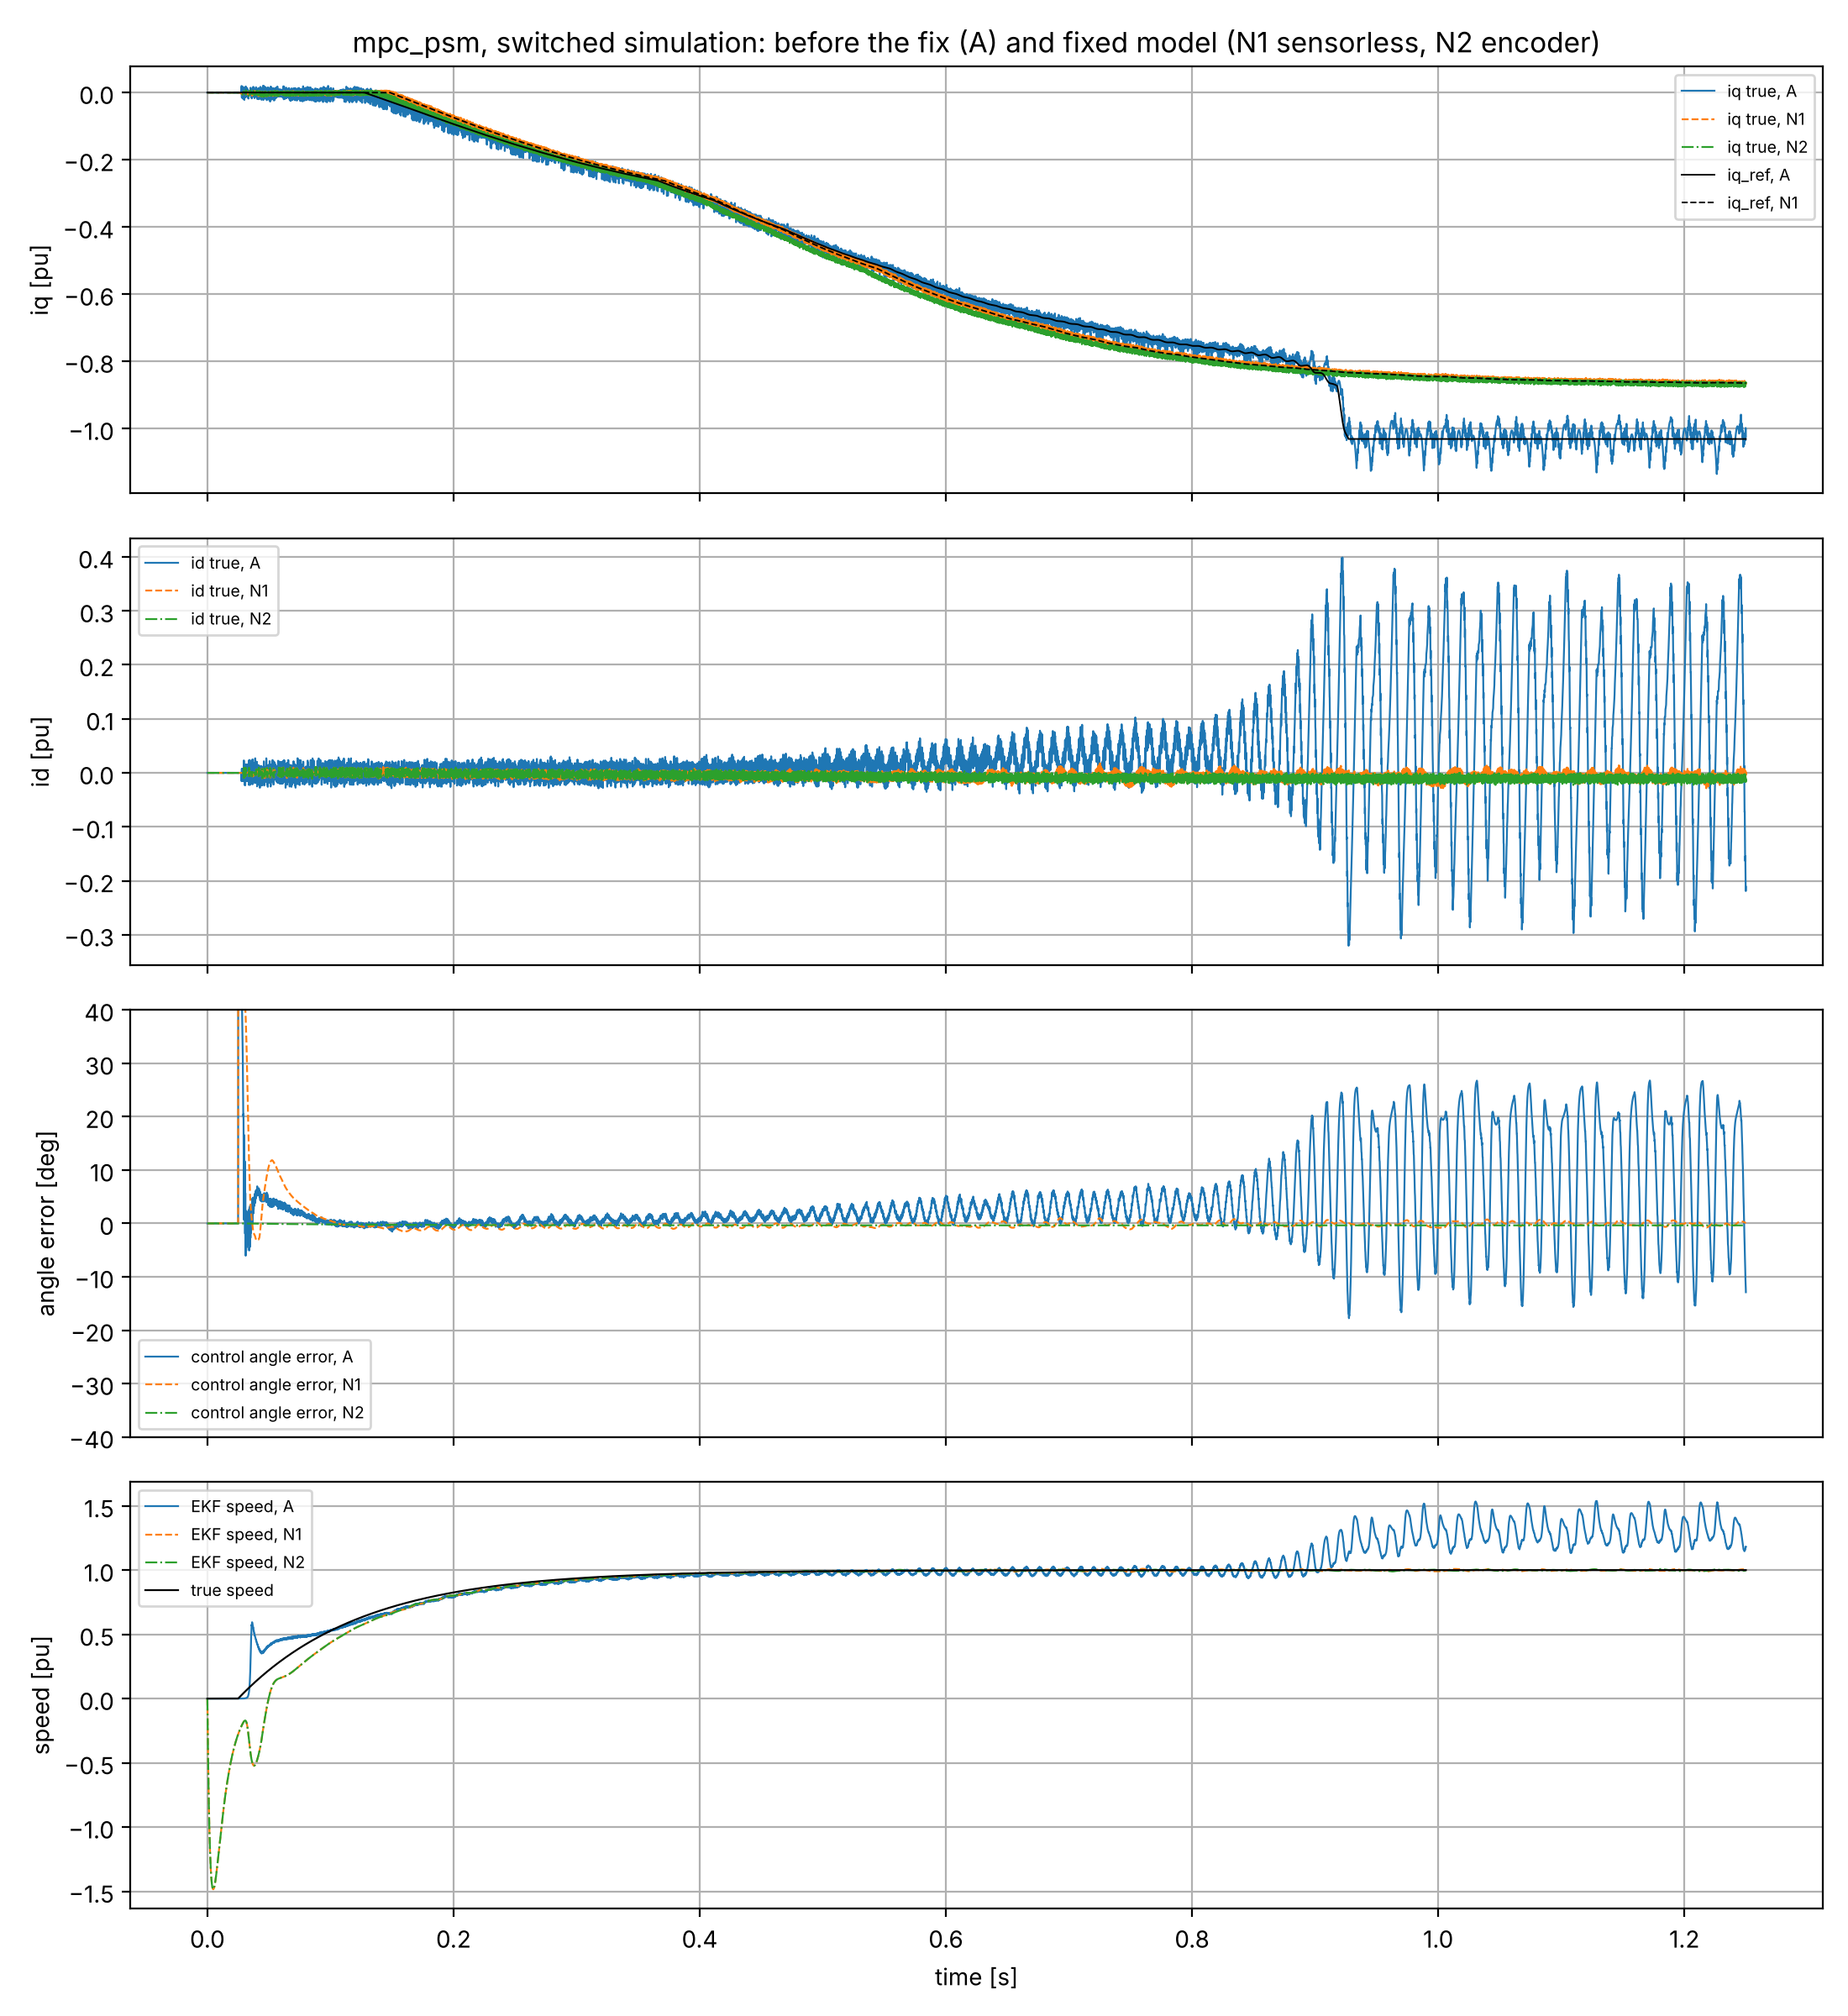
\includegraphics[width=0.82\textwidth]{figures/mpc_psm_startup.png}
	\caption{Start-up and rated operation in the switched simulation: $q$ and $d$ current, error of the control angle and speed of the control; model before the fix (A), fixed model sensorless (N1) and with the encoder (N2).}
	\label{fig:startup}
\end{figure}

\begin{figure}[H]
	\centering
	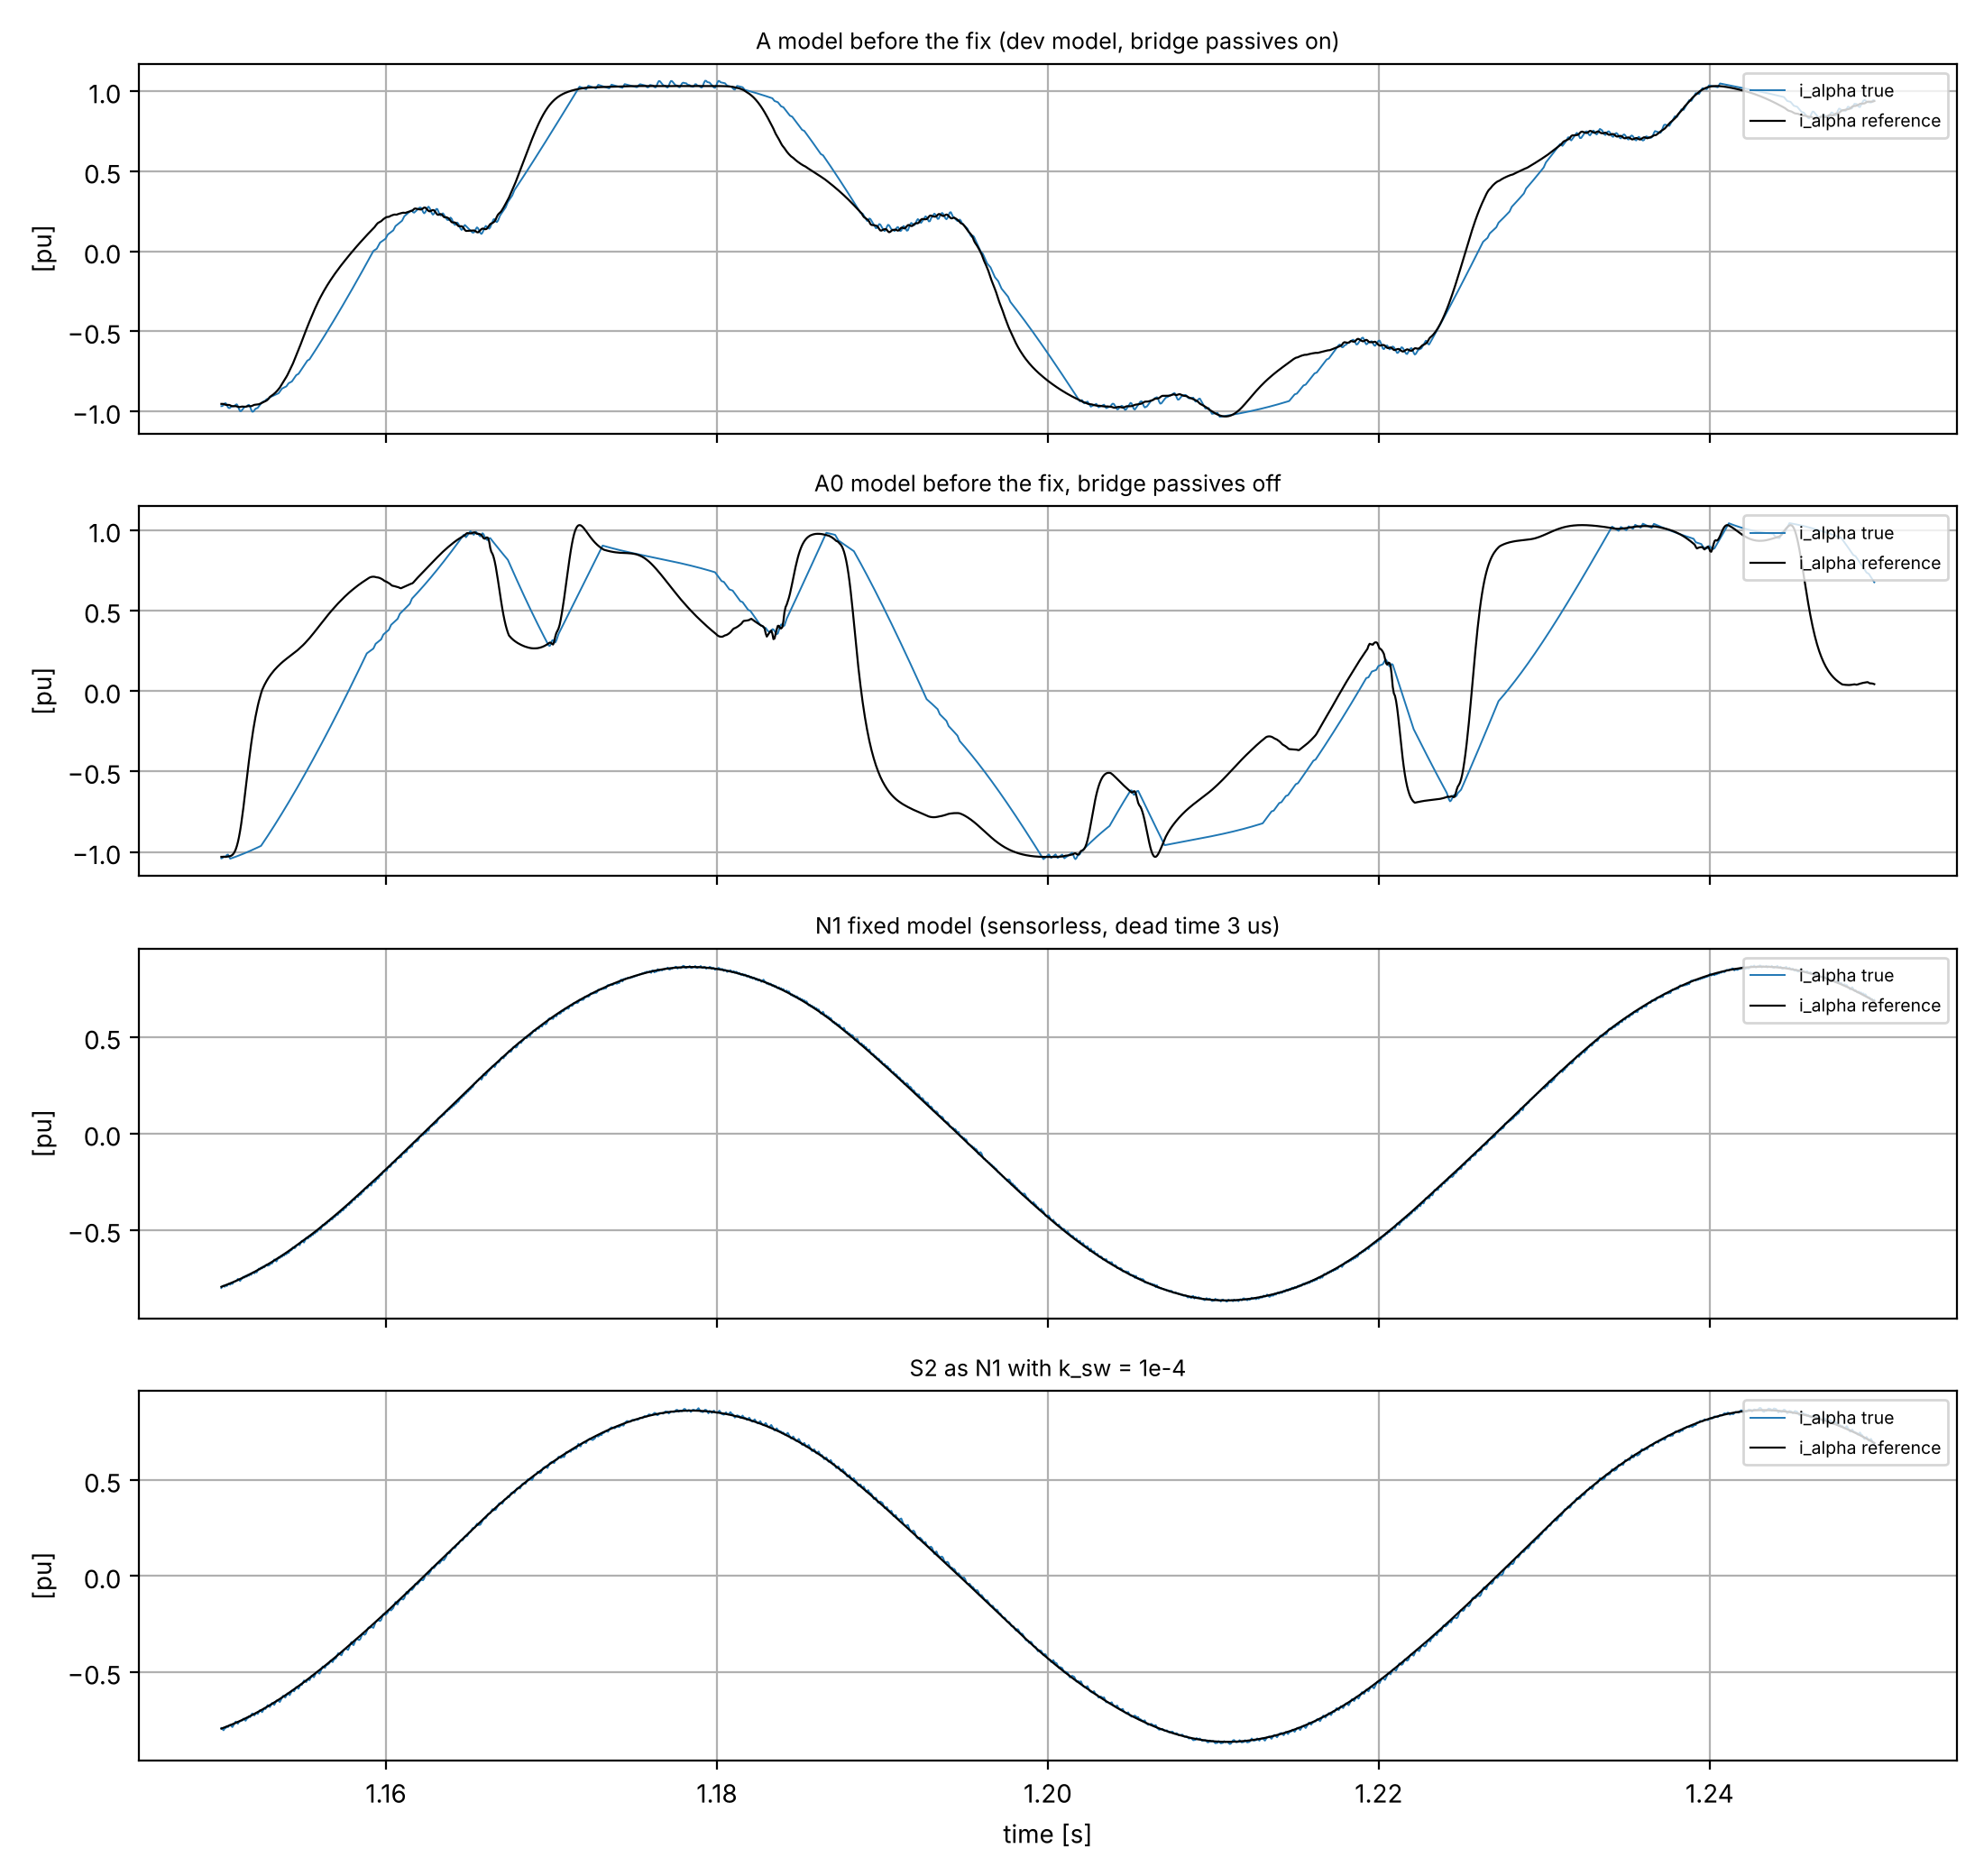
\includegraphics[width=0.82\textwidth]{figures/mpc_psm_current_zoom.png}
	\caption{Current $i_\alpha$ and its reference over \SI{100}{\milli\second} at rated speed: model before the fix with and without the bridge passives (A, A0), fixed model (N1) and fixed model with $k\ped{sw} = 10^{-4}$ (S2).}
	\label{fig:current}
\end{figure}

The check predicts for the scopes of the model: the current on its reference within about \SI{3}{\ampere} rms at rated power, the torque on the torque curve within the settling of the \SI{1}{\hertz} speed filter, the EKF angle within about \ang{0.5} of the encoder angle and the DC link at about \SI{1274}{\volt}.

% =============================================================
\section{What changed in November 2026}
\label{sec:history}

The model was migrated to the parameter structure \code{param} of the repository and its control was fixed in the same pull request (modelization-and-control PR \#33, merged into \code{dev} on 5 November 2026). Table~\ref{tab:fixes} lists the fixes; the README of the model gives the details of the migration (301 parameters re-pointed, 28 blocks without their Goto commented out, old and new names).

\begin{table}[H]
	\centering
	\footnotesize
	\caption{Control fixes of November 2026.}
	\label{tab:fixes}
	\rowcolors{2}{tableShade}{white}
	\begin{tabularx}{\textwidth}{@{} r X X @{}}
		\toprule
		\textbf{\#} & \textbf{Before} & \textbf{Now} \\
		\midrule
		1 & states computed from the constant $v\ped{dc} = 1$ in pu of $u\ped{dc,nom}$, in a model in pu of $u\ped{bez}$: the prediction saw the voltage 3.42 times too small & measured $v\ped{dc}$ times $k_u = 2.925$ (Section~\ref{sec:states}) \\
		2 & no delay compensation: unstable linear loop ($g = 3.0$ on $q$, 3.6 on $d$) & delay compensation, deadbeat on $q$ (Section~\ref{sec:deadbeat}) \\
		3 & 7 vectors, one zero vector, only neighbours after an active vector; switching term on the squared voltage with weight 0 & all 8 states; $k\ped{sw} = 10^{-5}$ times the legs that change state (Section~\ref{sec:cost}) \\
		4 & prediction with $L_s = (L_d + L_q)/2 = 0.889\pun$ and $R_s$, without the inductor & $L = L_q + L\ped{Fi} = 1.0033\pun$, $R = R_s + R\ped{LFi}$ (Section~\ref{sec:activeflux}) \\
		5 & EKF voltage 0.74 times the true one, of the vector chosen in the same step & $\underline{u}_{k-2}$ in pu of $u\ped{bez}$, gains 1 (Section~\ref{sec:ekftiming}) \\
		6 & EKF with $L_s$, $R_s$: \ang{-5.7} of angle at rated torque & $L$ and $R$ of fix 4: active flux \\
		7 & $A_6$ path of the state prediction without $\omega\ped{bez}$: speed about \SI{1}{\percent} low & \code{A6\_pred\_ekf} = 0 (Section~\ref{sec:ekfpred}) \\
		8 & speed output = speed state of the EKF, \SI{0.4}{\percent} low & speed from the DIO on the EKF angle (Section~\ref{sec:speed}) \\
		9 & EKF noise $q\ped{ekf} = 1/10$: angle lost at \SI{-15}{\percent} of the inductances & $q\ped{ekf} = 1/100$ \\
		10 & built-in passives of the new bridge block on: \SI{2}{\milli\farad} starting at \SI{0}{\volt} against the battery, \SI{1}{\milli\henry} per phase unknown to the control & passives off \\
		11 & the two back-EMF observers got 0.86 times the voltage, one step too new, with $L_s$, $R_s$ & same voltage, $L$ and $R$ as the EKF (not simulated) \\
		\bottomrule
	\end{tabularx}
\end{table}

% =============================================================
\section{Parameters}
\label{sec:params}

All numbers are in the structure \code{param} built by \code{init\_model.m}; Table~\ref{tab:params} lists those of the control. The README of the model describes every group of the structure.

\begin{table}[H]
	\centering
	\footnotesize
	\caption{Control parameters of \code{mpc\_psm} (\code{init\_model.m}, \code{private/psm\_ctrl\_param.m}).}
	\label{tab:params}
	\rowcolors{2}{tableShade}{white}
	\begin{tabularx}{\textwidth}{@{} >{\raggedright\arraybackslash}p{5.3cm} l X @{}}
		\toprule
		\textbf{Name} & \textbf{Value} & \textbf{Meaning} \\
		\midrule
		\code{param.time.fpwm}, \code{trgo} & \SI{15}{\kilo\hertz}, 0 & control timer, single update: $t\ped{s} = \SI{66.7}{\micro\second}$ (\code{param.glb\_time.ts\_inv}) \\
		\code{param.time.dead\_time} & \SI{3}{\micro\second} & dead time of the gate generator (\SI{2.94}{\micro\second} at the bridge) \\
		\code{param.inv.behav.}\newline\code{time\_gain\_module\_2} & 1.001 & gain of the control clock \code{time\_inv1} \\
		\code{param.psm.ctrl.mpc.u\_scale} & 2.9252 & $k_u = u\ped{dc,nom}/u\ped{bez}$ \\
		\code{param.psm.ctrl.mpc.L\_norm}, \code{R\_norm} & 1.0033, 0.0424 & $L = L_q + L\ped{Fi}$, $R = R_s + R\ped{LFi}$ (MPC, EKF, back-EMF observers) \\
		\code{param.psm.ctrl.mpc.k\_kalman}, \code{k\_sw} & 1, $10^{-5}$ & weights of the cost \eqref{eq:cost} \\
		\code{param.psm.ctrl.ekf.Qkalman} & \eqref{eq:noise} & $q\ped{ekf} = 1/100$, diagonal $[t\ped{s}^2\; t\ped{s}^2\; \frac12\; \frac12\; 1\; 1]$ \\
		\code{param.psm.ctrl.ekf.Rkalman} & $t\ped{s} I_2$ & $r\ped{ekf} = 1$ \\
		\code{param.psm.ctrl.ekf.A1\_tilde\_ekf} \ldots \code{A6\_tilde\_ekf}, \code{Bd\_ekf}, \code{C\_ekf} & Table~\ref{tab:jacobian} & EKF model with $j\ped{m} = 10^6$ (\code{jm\_ekf}); \code{Bd\_ekf} $= t\ped{s}B$ \\
		\code{param.psm.ctrl.ekf.A6\_pred\_ekf} & 0 & $A_6$ path of the state prediction \\
		\code{param.psm.ctrl.di\_obs.ktheta}, \code{komega} & 479.4, 36980 & DIO gains, poles $-1$ and $-4\,\omega\ped{bez}$ \\
		\code{param.psm.ctrl.kp\_w}, \code{ki\_w}, \code{iq\_lim} & 2.5, \SI{18}{\per\second}, 1.4 & speed PI (variant \code{use\_speed\_control}) \\
		\code{param.psm.ctrl.emf\_fb\_p}, \code{emf\_p}, \code{omega\_th} & 0.2, 0.08, 0 & back-EMF observers (variants), threshold of the encoder--sensorless switch \\
		\code{param.psm.u\_psm\_scale}, \code{u\_psm\_scale\_ekf} & 1, 1 & voltage scale of the observers (the voltage is already in pu of $u\ped{bez}$) \\
		\code{param.psm.mode.use\_torque\_curve}, \code{use\_psm\_encoder} & 1, 0 & torque curve, sensorless \\
		\code{param.psm.impl.}\newline\code{use\_ekf\_bemf\_module\_1} & 1 & EKF active (the two back-EMF observers are variants) \\
		\code{param.load.rpm\_base}, \code{torque\_base} & Figure~\ref{fig:torquecurve} & torque curve per system; \code{torque\_overload\_factor} = 1 \\
		\code{param.ctrl.filters.inv.g0\_1Hz}, \code{g1\_1Hz} & $4.19\cdot10^{-4}$ & \SI{1}{\hertz} speed filter of the torque curve \\
		\code{param.meas.adc\_quantization} & $2^{-11}$ & quantization of the acquisitions (pu) \\
		\code{param.ctrl.kp\_align}, \code{ki\_align} & 0.25, \SI{18}{\per\second} & alignment loop of the clock (its mask has gains 0, open point~\ref{op:clock}) \\
		\code{param.sim.simlength}, \code{nonlinear\_iterations} & \SI{1.25}{\second}, 5 & stop time, Simscape nonlinear iterations \\
		\bottomrule
	\end{tabularx}
\end{table}

% =============================================================
\section{Files and how to run the model}
\label{sec:files}

\textbf{How to run.} (1) Clone the \code{library} repository next to \code{modelization-and-control} (or set the environment variable \code{PWR\_CONTROL\_LIBRARY}): the function \code{library\_setup} of the model puts it on the MATLAB path and clones it when it is missing. (2) From the folder \code{foundations\_of\_power\_electronics/mpc\_psm} run \code{init\_model.m}: it fills \code{param}, prints the bases and the design figures, opens \code{mpc\_psm.slx}, sets the mechanical setting and checks that every \code{param.*} name read by the model exists and that every active From has its Goto. (3) Run the simulation (\SI{1.25}{\second}).

\begin{table}[H]
	\centering
	\footnotesize
	\caption{Files of the model and of this note.}
	\label{tab:files}
	\rowcolors{2}{tableShade}{white}
	\begin{tabularx}{\textwidth}{@{} >{\raggedright\arraybackslash}p{5.0cm} X @{}}
		\toprule
		\textbf{File} & \textbf{Content} \\
		\midrule
		\multicolumn{2}{@{}>{\raggedright\arraybackslash}p{\dimexpr\textwidth-2\tabcolsep\relax}@{}}{\textbf{model \code{foundations\_of\_power\_electronics/mpc\_psm/} of \code{pwr-control/modelization-and-control} (branch \code{dev})}} \\
		\code{init\_model.m} & initialization as a plain-text live script: every number in \code{param}, design figures, model checks \\
		\code{mpc\_psm.slx} & the model: power stage, machine, control, logging \\
		\code{mpc\_psm\_private.m}, \code{private/} & handles to the parameter functions (\code{timing\_param}, \code{inv\_hw\_param}, \code{psm\_machine\_param}, \code{psm\_ctrl\_param}, \code{battery\_param}, \code{library\_setup}, the two model checks) \\
		\code{README.md} & model, parameters, control fixes, migration, checks, design figures, open points \\
		\code{spectrum.m} & FFT of a phase current of the machine and of a phase voltage \\
		\midrule
		\multicolumn{2}{@{}>{\raggedright\arraybackslash}p{\dimexpr\textwidth-2\tabcolsep\relax}@{}}{\textbf{this note, \code{repos\_doc/psm\_mpc\_ekf/} of \code{pwr-control/repositories-documentation}}} \\
		\code{psm\_mpc\_ekf.tex}, \code{.pdf} & source and PDF \\
		\code{py/design\_check\_mpc\_psm.py} & switched simulation of the whole chain (Section~\ref{sec:check}): writes \code{figures/design\_check\_mpc\_psm\_output.txt} and the two PNG figures; run \code{python3 design\_check\_mpc\_psm.py ../figures} from \code{py/} (about two minutes) \\
		\code{py/mpc\_port\_2l.py} & Python copies of the function \code{mpc} (fixed and old), used by the check \\
		\code{py/ekf\_speed\_bias.py} & isolated test of the EKF (Table~\ref{tab:bias}); its output is \code{figures/ekf\_speed\_bias\_output.txt} \\
		\code{figures/} & the outputs of the two scripts \\
		\bottomrule
	\end{tabularx}
\end{table}

% =============================================================
\section{Open points}
\label{sec:open}

\begin{enumerate}[nosep]
	\item \label{op:matlab} \textbf{Check in MATLAB.} The fixes were designed with the switched simulation and the init was checked in Octave; a run of the model in MATLAB should show the scopes listed at the end of Section~\ref{sec:check}.
	\item \label{op:clock} \textbf{Clock.} The control clock \code{time\_inv1} has the gain 1.001 (\SI{15015}{\hertz}) while the constants use \SI{66.7}{\micro\second}: the prediction step is \SI{0.1}{\percent} short and the speed is 0.999. Harmless here (no carrier), but it is the last error of the speed. The alignment loop \code{phase\_compensation\_1/alignment\_ctrl} feeds this clock but has $k_p = k_i = 0$ typed in its mask.
	\item \label{op:range} \textbf{Sensorless range.} The angle error grows by about \ang{0.47} per percent of error of the machine inductances (Section~\ref{sec:ekf}); the angle is held from \SI{-25}{\percent} to \SI{+20}{\percent}. If the real inductances are not known within about \SI{\pm 10}{\percent}, an adaptation of the inductance or of the angle is needed, or the encoder.
	\item \label{op:angle} \textbf{Age of the control angle.} Three steps, \ang{1.1} at rated speed, $i_d \approx -0.017\pun$ (Section~\ref{sec:reference}). An angle advance of $3\,\omega h$ in the current reference would remove it.
	\item \textbf{DC voltage.} The battery holds the DC link at 1249--\SI{1274}{\volt}, 1.17--1.19 times $u\ped{dc,nom}$ of the \SI{690}{\volt} data set: the voltage rating of the switches should be checked. The control uses the measured DC voltage and follows the battery.
	\item \textbf{Battery capacity.} The init uses $P/V = \SI{208}{\ampere\hour}$ (1C) as an assumption; it does not matter in \SI{1.25}{\second}.
	\item \textbf{Simulation length.} \SI{1.25}{\second} ends while the \SI{1}{\hertz} speed filter is still settling (\SI{-1.3}{\percent} of torque); \SI{2}{\second} would show the steady state.
	\item \label{op:start} \textbf{Start of the speed estimate.} The DIO of the EKF block starts at $\theta\ped{o} = \pi$ while the EKF angle starts elsewhere: at standstill its speed swings down to about \SI{-1.5}{} pu (at \SI{5}{\milli\second}, Figure~\ref{fig:startup}) and follows the true speed from about \SI{0.15}{\second}. The flux of the EKF is about zero at standstill and the torque reference is zero below \SI{4}{rpm}, so the current is not disturbed, but the scopes show it.
	\item \label{op:torque} \textbf{Torque row of the state prediction.} With \code{A6\_pred\_ekf} = 0 the speed row of $F\ped{pred}$ counts the torque products twice (Section~\ref{sec:ekfpred}). It has no effect with $j\ped{m} = 10^6$; with a real inertia in the EKF model one of the two pairs ($A_2$, $A_3$ or the $1/j\ped{m}$ entries of $A_4$, $A_5$) should be left out of the prediction copy.
	\item \textbf{Not checked.} The speed-control variant and the two back-EMF observers (fixed by construction, not simulated); the post-processing scripts \code{plotting\_results\_inv.m} and \code{power\_losses\_calculus.m} of the model folder come from other models and do not run on this one.
\end{enumerate}

% =============================================================
\begin{thebibliography}{99}
	\bibitem{mc_repo} pwr-control, \textit{modelization-and-control} repository, model \path{foundations_of_power_electronics/mpc_psm} (branch \code{dev}) and its README, \url{https://github.com/pwr-control/modelization-and-control}.
	\bibitem{library_repo} pwr-control, \textit{library} repository (bridge, DC link, battery and machine blocks; \code{ekf\_pmsm\_setup}, \code{ctrl\_pmsm\_setup}), \url{https://github.com/pwr-control/library}.
	\bibitem{kouro2009} S.~Kouro, P.~Cort\'es, R.~Vargas, U.~Ammann, and J.~Rodr\'iguez, ``Model predictive control---a simple and powerful method to control power converters,'' \emph{IEEE Trans. Ind. Electron.}, vol.~56, no.~6, pp.~1826--1838, June 2009.
	\bibitem{rodriguez2012} J.~Rodr\'iguez and P.~Cort\'es, \emph{Predictive Control of Power Converters and Electrical Drives}. Wiley--IEEE Press, 2012.
	\bibitem{cortes2012} P.~Cort\'es, J.~Rodr\'iguez, C.~Silva, and A.~Flores, ``Delay compensation in model predictive current control of a three-phase inverter,'' \emph{IEEE Trans. Ind. Electron.}, vol.~59, no.~2, pp.~1323--1325, Feb. 2012.
	\bibitem{boldea2008} I.~Boldea, M.~C. Paicu, and G.-D. Andreescu, ``Active flux concept for motion-sensorless unified AC drives,'' \emph{IEEE Trans. Power Electron.}, vol.~23, no.~5, pp.~2612--2618, Sept. 2008.
	\bibitem{bolognani2003} S.~Bolognani, L.~Tubiana, and M.~Zigliotto, ``Extended Kalman filter tuning in sensorless PMSM drives,'' \emph{IEEE Trans. Ind. Appl.}, vol.~39, no.~6, pp.~1741--1747, Nov./Dec. 2003.
	\bibitem{simon2006} D.~Simon, \emph{Optimal State Estimation: Kalman, $H_\infty$, and Nonlinear Approaches}. Wiley, 2006.
	\bibitem{ttype_note} D.~Bagnara, \textit{Finite-set predictive current control of a T-type wind-generator inverter: analysis and fixes of the model \code{mpc\_ttype\_psm}}, pwr-control technical note, Rev.~00, November 2026, \path{research/power_electronics/fcs_mpc_ttype_psm} of \url{https://github.com/pwr-control/repositories-documentation}.
	\bibitem{psm_note} D.~Bagnara, \textit{Permanent Magnet Synchronous Machines: model derivation, control and Simscape implementation}, pwr-control report, May 2021, \path{repos_doc/psm_model_observer_ctrl} of \url{https://github.com/pwr-control/repositories-documentation}.
\end{thebibliography}

% =============================================================
\clearpage
\appendix
\section{The function \code{mpc} of the model}
\label{app:mpc}

The MATLAB Function \code{mpc} of the block \code{inner\_ctrl/mp control/mpc\_pu\_d} of \code{mpc\_psm.slx} (chart 58), as it is in the model since November 2026. The inputs come from Constants that read \code{param.psm.ctrl.mpc.*}, \code{param.psm.machine.omega\_bez} and \code{param.glb\_time.ts\_inv}; \code{vdc} comes from the From \code{udcd\_pu\_inv\_mod1}.

\begin{singlespace}
\fontsize{7.5}{9}\selectfont
\begin{verbatim}
function [ualpha, ubeta, cmg_g1, cmg_g2, cmg_g3, cmg_g4, cmg_g5, cmg_g6] = mpc(vdc, ialpha_ref, ...
    ibeta_ref, ialpha, ibeta, omega_hat, psi_alpha_hat, psi_beta_hat, u_scale, ...
    L_norm, omega_bez, R_norm, k_kalman, k_sw, ts_inv)
% Finite-set predictive current control of the two-level bridge: every control step it tests the 8 states
% of the bridge and applies the one with the lowest cost (current error and switching).
%
% Inputs, all per unit of the machine:
%   vdc                     DC-link voltage measured one control step before, pu of udc_nom
%   ialpha_ref, ibeta_ref   current reference, pu of ibez
%   ialpha, ibeta           current measured one control step before, pu of ibez
%   omega_hat               speed of the EKF block, pu of omega_bez
%   psi_alpha_hat, psi_beta_hat   flux of the EKF, pu of psi_m
%   u_scale                 udc_nom/ubez: voltage in pu of udc_nom -> voltage in pu of ubez
%   L_norm, R_norm          inductance and resistance seen by the bridge: q axis of the machine plus the output
%                           inductor, pu of the machine (the EKF uses the same values)
%   omega_bez               [rad/s] electrical base pulsation
%   k_kalman, k_sw          weights of the current error and of the number of legs that change state
%   ts_inv                  [s] control step
% Outputs:
%   ualpha, ubeta           voltage of the vector applied in the last step, pu of ubez. The Unit Delay after
%                           this block makes it the vector of two steps before: the vector that acted before the
%                           current measured one step before, the pair the EKF needs.
%   cmg_g1 ... cmg_g6       gate commands (0 or 15 V) of a+, a-, b+, b-, c+, c- (the dead time is added in
%                           the inverter by the gate generator)
%
% Timing: current and DC voltage are measured one control step before, and the vector chosen now acts until
% the next step. So the control first computes the current of now with the vector of the last step (delay
% compensation), then chooses the vector for the next step.

    persistent states_table u_last s_last

    if isempty(states_table)
        % the 8 states [leg a, leg b, leg c]: 1 = upper switch on, 0 = lower switch on
        states_table = [0 0 0; 1 0 0; 1 1 0; 0 1 0; 0 1 1; 0 0 1; 1 0 1; 1 1 1];
        u_last = [0; 0];            % voltage of the vector applied in the last step, pu of ubez
        s_last = [0 0 0];           % legs of the vector applied in the last step
    end

    Vdd = 15;
    inv_sqrt3 = 0.577350269189626;
    ts_pu = ts_inv*omega_bez;
    g = ts_pu/L_norm;

    % back-EMF of the EKF flux, e = d(psi)/dt = j*omega*psi (pu of ubez)
    ealpha = -omega_hat*psi_beta_hat;
    ebeta = omega_hat*psi_alpha_hat;

    % 1. Delay compensation: current of now, from the current measured one step before and the vector
    %    applied since then
    ialpha0 = ialpha + g*(u_last(1) - R_norm*ialpha - ealpha);
    ibeta0 = ibeta + g*(u_last(2) - R_norm*ibeta - ebeta);

    % 2. Prediction and cost of the 8 states (the first state with the lowest cost wins)
    minJ = 1e18;
    best_idx = 1;
    ua_best = 0.0;
    ub_best = 0.0;

    for n = 1:8
        sa = states_table(n,1);
        sb = states_table(n,2);
        sc = states_table(n,3);

        % alpha/beta voltage of the state, pu of ubez (leg voltages sa*vdc, sb*vdc, sc*vdc)
        ua = u_scale*vdc*(sa - 0.5*sb - 0.5*sc)*2/3;
        ub = u_scale*vdc*(sb - sc)*inv_sqrt3;

        % current at the next step
        ia_p = ialpha0 + g*(ua - R_norm*ialpha0 - ealpha);
        ib_p = ibeta0 + g*(ub - R_norm*ibeta0 - ebeta);

        % legs that change state from the vector of the last step
        nsw = abs(sa - s_last(1)) + abs(sb - s_last(2)) + abs(sc - s_last(3));

        % cost
        J = k_kalman*((ialpha_ref - ia_p)^2 + (ibeta_ref - ib_p)^2) + k_sw*nsw;

        if J < minJ
            minJ = J;
            best_idx = n;
            ua_best = ua;
            ub_best = ub;
        end
    end

    % 3. Voltage for the observers (vector of the last step), then the memory of the applied vector
    ualpha = u_last(1);
    ubeta = u_last(2);
    u_last = [ua_best; ub_best];
    s_last = states_table(best_idx, :);

    % 4. Gate commands of the chosen state
    ga = states_table(best_idx, 1);
    gb = states_table(best_idx, 2);
    gc = states_table(best_idx, 3);

    cmg_g1 = Vdd*ga;
    cmg_g2 = Vdd*(1 - ga);
    cmg_g3 = Vdd*gb;
    cmg_g4 = Vdd*(1 - gb);
    cmg_g5 = Vdd*gc;
    cmg_g6 = Vdd*(1 - gc);
end
\end{verbatim}
\end{singlespace}

\end{onehalfspace}
\end{document}
